%%
%% This is file `sample-sigconf.tex',
%% generated with the docstrip utility.
%%
%% The original source files were:
%%
%% samples.dtx  (with options: `sigconf')
%% 
%% IMPORTANT NOTICE:
%% 
%% For the copyright see the source file.
%% 
%% Any modified versions of this file must be renamed
%% with new filenames distinct from sample-sigconf.tex.
%% 
%% For distribution of the original source see the terms
%% for copying and modification in the file samples.dtx.
%% 
%% This generated file may be distributed as long as the
%% original source files, as listed above, are part of the
%% same distribution. (The sources need not necessarily be
%% in the same archive or directory.)
%%
%% Commands for TeXCount
%TC:macro \cite [option:text,text]
%TC:macro \citep [option:text,text]
%TC:macro \citet [option:text,text]
%TC:envir table 0 1
%TC:envir table* 0 1
%TC:envir tabular [ignore] word
%TC:envir displaymath 0 word
%TC:envir math 0 word
%TC:envir comment 0 0
%%
%%
%% The first command in your LaTeX source must be the \documentclass command.


% Fixing: Too many math alphabets used in version normal.
\newcommand\hmmax{0}
\newcommand\bmmax{0}
\documentclass[utf8,acmsmall,review,screen,dvipsnames]{acmart}

\usepackage[colorinlistoftodos]{todonotes}
\usepackage[inference]{semantic}
\usepackage{fontawesome5}
\usepackage{listofitems}
\usepackage{glossaries}
\usepackage{cleveref}
\usepackage{stmaryrd}
\usepackage{marvosym}
\usepackage{listings}
\usepackage{xspace}
\usepackage{xfrac}
\usepackage{tikz}
\usepackage{soul}
\usepackage{bm}

\setul{0.5ex}{0.3ex}

% https://tex.stackexchange.com/questions/648845/sans-serif-uppercase-greek-no-longer-showing-in-acmart
\DeclareMathAlphabet{\mathsf}{OT1}{LibertinusSans-LF}{m}{n}
\SetMathAlphabet{\mathsf}{bold}{OT1}{LibertinusSans-LF}{bx}{n}

\DeclareMathAlphabet{\mathtt}{OT1}{lmtt}{m}{n}
\SetMathAlphabet{\mathtt}{bold}{OT1}{lmtt}{bx}{n}


\usetikzlibrary{calc,decorations.pathmorphing,shapes,positioning}
\newcounter{sarrow}
\newcommand\xrsquigarrow[1]{%
\stepcounter{sarrow}%
\mathrel{\begin{tikzpicture}[baseline= {( $ (current bounding box.south) + (0,-0.5ex) $ )}]
\node[inner sep=.5ex] (\thesarrow) {$\scriptstyle #1$};
\path[draw,<-,decorate,
  decoration={zigzag,amplitude=0.7pt,segment length=1.2mm,pre=lineto,pre length=4pt}]
    (\thesarrow.south east) -- (\thesarrow.south west);
\end{tikzpicture}}%
}
\makeatletter
\newcommand{\xRightarrow}[2][]{\ext@arrow 0359\Rightarrowfill@{#1}{#2}}
\makeatother

\newcommand{\thmref}[1]{\cref{#1}~(\nameref{#1})}
\newcommand{\Thmref}[1]{\Cref{#1}~(\nameref{#1})}

%%%%
% TODO macros
\newcommand{\MK}[1]{\todo[color=orange!30]{TODO: #1}}
\newcommand{\MKin}[1]{\todo[color=orange!30,inline]{TODO: #1}}
\newcommand{\MP}[1]{\todo[color=blue!30]{TODO: #1}}
\newcommand{\MPin}[1]{\todo[color=blue!30,inline]{TODO: #1}}
\newcommand{\hltt}[1]{\begin{center}\fbox{\color{green}\large{#1}}\end{center}}

% Approx
\newcommand{\pages}[1]{}%\xspace\todo{\textbf{($\sim$#1 pages)}\xspace}}

%%%%
% Colors
\newcommand{\neutcol}[0]{black}
\newcommand{\stlccol}[0]{RoyalBlue}
\newcommand{\irccol}[0]{Apricot}
\newcommand{\ulccol}[0]{RedOrange}
\newcommand{\objcol}[0]{Emerald} %CarnationPink}
\newcommand{\commoncol}[0]{black}

\newcommand{\col}[2]{\ensuremath{{\color{#1}{#2}}}}

\newcommand{\com}[1]{\ensuremath\mathit{\col{\neutcol}{#1}}}
\newcommand{\src}[1]{\ensuremath\mathsf{\col{\stlccol}{#1}}}
\newcommand{\irl}[1]{\ensuremath\mathit{\col{\irccol}{#1}}}
\newcommand{\trg}[1]{\ensuremath\mathbf{\col{\ulccol}{#1}}}
\newcommand{\obj}[1]{\ensuremath\mathtt{\col{\objcol}{#1}}}

%%%%
% Text Decorations
\newcommand\BrText[2]{%
  \par\smallskip
   \noindent\makebox[\textwidth][r]{$\text{\scriptsize #1}\left\{
    \begin{minipage}{\textwidth}
    #2
    \end{minipage}
  \right.\nulldelimiterspace=0pt$}\par\smallskip
}
\newcommand{\mi}[1]{\ensuremath{\mathit{#1}}}
\newcommand{\mr}[1]{\ensuremath{\mathrm{#1}}}
\newcommand{\mt}[1]{\ensuremath{\texttt{#1}}}
\newcommand{\mtt}[1]{\ensuremath{\mathtt{#1}}}
\newcommand{\mf}[1]{\ensuremath{\mathbf{#1}}}
\newcommand{\mk}[1]{\ensuremath{\mathfrak{#1}}}
\newcommand{\mc}[1]{\ensuremath{\mathcal{#1}}}
\newcommand{\ms}[1]{\ensuremath{\mathsf{#1}}}
\newcommand{\mb}[1]{\ensuremath{\mathbb{#1}}}
\newcommand{\msc}[1]{\ensuremath{\mathscr{#1}}}

\newcommand{\bul}[1]{{\setulcolor{RoyalBlue}\ul{#1}}}
\newcommand{\rul}[1]{{\setulcolor{RedOrange}\ul{#1}}}
\newcommand{\iul}[1]{{\setulcolor{Apricot}\ul{#1}}}
\newcommand{\oul}[1]{{\setulcolor{Emerald}\ul{#1}}}
\newcommand{\pul}[1]{{\setulcolor{CarnationPink}\ul{#1}}}

\newcommand{\lock}{\ensuremath\text{\scriptsize\faIcon{lock}}}
\newcommand{\unlock}{\ensuremath\text{\scriptsize\faIcon{lock-open}}}

\newcommand{\tup}[2]{\ensuremath (#1 %
  \readlist\myterms{#2}%
  \foreachitem\x\in\myterms{;\x}%
  )%
}

\newcommand{\isdef}[0]{\ensuremath{\mathrel{\overset{\makebox[0pt]{\mbox{\normalfont\tiny\sffamily def}}}{=}}}}

%%%%
% List of contributions
\newcounter{contrib}
\newcommand{\contribnum}[0]{\stepcounter{contrib}{\arabic{contrib}}.~}
\newcommand{\contribution}[1]{\smallskip\noindent\textbf{{#1.}\xspace}}

%%%%
% A symbol for Coq-verified theorems.
\newcommand{\BareCoqSymbol}{
\includegraphics[height=0.9em]{coq.pdf}}
\newcommand{\CoqSymbol}{\raisebox{-.2ex}{\BareCoqSymbol\,}}
\newcommand{\Coqed}{\hfill\CoqSymbol}

\newcommand{\BareInvCoqSymbol}{
\includegraphics[height=0.9em]{inv_coq.png}}
\newcommand{\InvCoqSymbol}{\raisebox{-.2ex}{\BareInvCoqSymbol\,}}

%%%%
% Typerules
\newcommand{\textgraybox}[1]{\boxed{#1}}
\newdimen\zzfontsz
\newcommand{\fontsz}[2]{\zzfontsz=#1%
{\fontsize{\zzfontsz}{1.2\zzfontsz}\selectfont{#2}}}
\newcommand{\mathsz}[2]{\text{\fontsz{#1}{$#2$}}}
\newcommand{\instsymColon}{%
     \raisebox{-0.09ex}{\text{\normalfont{:}}}}
\newcommand{\judgboxfontsize}[1]{%
        \mathsz{11pt}{#1}%
}
\newcommand{\judgbox}[2]{%
      {\raggedright \textgraybox{\ensuremath{\judgboxfontsize{#1}}}\!%
        \fontsz{9pt}{\begin{tabular}[c]{l} #2 \end{tabular}} %
}}
\newcounter{typerule}
\crefname{typerule}{rule}{rules}

\newcommand{\typeruleInt}[5]{%
	\def\thetyperule{#1}%
	\refstepcounter{typerule}%
	\label{tr:#4}%
	%
  \ensuremath{\begin{array}{c}#5 \inference{#2}{#3}\end{array}}
}
\newcommand{\typerule}[4]{%
  \typeruleInt{#1}{#2}{#3}{#4}{\textsf{\scriptsize ({#1})} \\      }
}
\newcommand{\typerulenolabel}[3]{%
	\def\thetyperule{#1}%
	\refstepcounter{typerule}%
  \ensuremath{\begin{array}{c} \inference{#2}{#3}\end{array}}
}
\newcommand{\typerulederiv}[3]{%
  \ensuremath{\begin{array}{c} \inference{#2}{#3} #1\end{array}}
}

%%%%
% Language-specific definitions
% names of properties
\newcommand{\tmssafe}{\ensuremath\operatorname{tms}}
\newcommand{\smssafe}{\ensuremath\operatorname{sms}}
\newcommand{\mssafe}{\ensuremath\operatorname{ms}}
\newcommand{\scctsafe}{\ensuremath\operatorname{scct}}
\newcommand{\msscctsafe}{\ensuremath\operatorname{msscct}}

% Languages
\newcommand{\Ltms}{\ensuremath\src{L_{\tmssafe}}}
\newcommand{\Ltrg}{\ensuremath\trg{L}}
\newcommand{\Lms}{\ensuremath\irl{L_{\mssafe}}}
\newcommand{\Lscct}{\ensuremath\obj{L_{\scctsafe}}}

% Traces
\newcommand{\event}[1][]{a#1}
\newcommand{\absevent}[1][]{\ensuremath\bm{\event[#1]}}
\newcommand{\emptyevent}{\ensuremath\varepsilon}
\newcommand{\trace}[1][]{\ensuremath\overline{a#1}}
\newcommand{\class}[1][]{\ensuremath\mb{C}}
\newcommand{\lift}[1]{\ensuremath\lfloor\xspace{#1}\xspace\rfloor}
\newcommand{\hole}[1]{\ensuremath{\left[#1\right]}}
\newcommand{\ev}[1]{\text{#1}}
\newcommand{\absev}[1]{\ensuremath\bm{#1}}
\newcommand{\abstrace}[1][]{\ensuremath\bm{\trace[]}#1}
\newcommand{\absterm}{\ensuremath\lightning{\kern-5.5pt}\lightning}

% Trace Relations
\newcommand{\traceagree}[4][^*]{\ensuremath{#3}\cong_{#2}#1{#4}}
\newcommand{\tmstraceagree}[3][^*]{\traceagree[#1]{\tmssafe}{#2}{#3}}
\newcommand{\smstraceagree}[3][^*]{\traceagree[#1]{\smssafe}{#2}{#3}}
\newcommand{\mstraceagree}[3][^*]{\traceagree[#1]{\mssafe}{#2}{#3}}
\newcommand{\sccttraceagree}[3][^*]{\traceagree[#1]{\scctsafe}{#2}{#3}}

% Monitors
\newcommand{\monitor}[1][]{\ensuremath T#1}
\newcommand{\tmsmonitor}[1][]{\monitor[_{TMS}{#1}]}
\newcommand{\smsmonitor}[1][]{\monitor[_{SMS}{#1}]}
\newcommand{\scctmonitor}[1][]{\monitor[_{sCCT}{#1}]}
\newcommand{\msmonitor}[1][]{\monitor[_{MS}{#1}]}
\newcommand{\monitorcheck}[4][{\kern-3.5pt}^*]{%
  \vdash\xspace{#2}\xspace \xrsquigarrow{#4}{#1}\xspace{#3}\xspace%
}
\newcommand{\monsafe}[2]{\ensuremath\vdash_{mon}{#1}:{#2}}

\newcommand{\abssecuritytag}[1][]{\ensuremath\bm{\sigma}#1}

\newcommand{\montmssafe}[1]{\monsafe{#1}{\tmssafe}}
\newcommand{\monsmssafe}[1]{\monsafe{#1}{\smssafe}}
\newcommand{\monmssafe}[1]{\monsafe{#1}{\mssafe}}
\newcommand{\monscctsafe}[1]{\monsafe{#1}{\scctsafe}}
\newcommand{\monmsscctsafe}[1]{\monsafe{#1}{\msscctsafe}}

% Languages
\newcommand{\LTMS}{\src{L_{TMS}}}
\newcommand{\LT}{\trg{L}}
\newcommand{\LMS}{\irl{L_{MS}}}
\newcommand{\LCCT}{\obj{L_{sCCT}}}

\newcommand{\bnfdef}{\ensuremath{\mathrel{::=}}}

% Substitution
\newcommand{\subst}[2]{\ensuremath \hole{#1\text{ for }#2}}
\newcommand{\substvar}[1][]{\ensuremath \gamma#1}
\newcommand{\substlist}[1][]{\ensuremath \overline{\gamma#1}}

\newcommand{\partialeval}[2]{\ensuremath \operatorname{\mathtt{mix}}(#1, #2)}

% Predefined Sets
\newcommand{\nat}{\ensuremath\mb{N}}

% Types
\newcommand{\natt}{\ensuremath\mb{N}_t\xspace}
\newcommand{\ptrqual}[1][]{\ensuremath\xspace q#1\xspace}
\newcommand{\fullq}{1\xspace}
\newcommand{\halfq}{\sfrac{1}{2}\xspace}
\newcommand{\ptrn}[1][\ptrqual]{\ensuremath\xspace ref_{#1}\ \natt\xspace}
\newcommand{\wptr}{\ensuremath\ptrn[\halfq]\xspace}
\newcommand{\ptr}{\ensuremath\ptrn[\fullq]\xspace}
\newcommand{\type}[1][]{\ensuremath\tau#1\xspace}
\newcommand{\typenv}[1][]{\ensuremath\Gamma#1\xspace}

% Terms
\newcommand{\wrapkeyword}[2][]{\ensuremath{#1{#2}}}
\newcommand{\expr}[1][]{e#1\xspace}
\newcommand{\ectx}[1][]{K#1\xspace}
\newcommand{\finalexpr}[1][]{f#1\xspace}
\newcommand{\valueexpr}[1][]{v#1\xspace}
\newcommand{\lbinop}[3][]{\ensuremath {#2}{#1{\oplus}}{#3}\xspace}
\newcommand{\lget}[3][]{\ensuremath #2{#1{[}}{#3}{#1{]}}\xspace}
\newcommand{\lset}[4][]{\ensuremath #2{#1{[}}{#3}{#1{]\leftarrow}}#4\xspace}
\newcommand{\lnew}[3][]{\ensuremath \wrapkeyword[#1]{new}\ #2\ {#1{[}}#3{#1{]}}\xspace}
\newcommand{\llet}[4][]{\ensuremath \wrapkeyword[#1]{let}\ #2 {#1{=}} #3\ \wrapkeyword[#1]{in}\ #4\xspace}
\newcommand{\ldelete}[2][]{\ensuremath \wrapkeyword[#1]{delete}\ #2\xspace}
\newcommand{\lreturn}[2][]{\ensuremath \wrapkeyword[#1]{return}\ #2\xspace}
\newcommand{\lcall}[3][]{\ensuremath \wrapkeyword[#1]{call}\ #2\ #3\xspace}
\newcommand{\lifz}[4][]{\ensuremath \wrapkeyword[#1]{ifz}\ #2\ \wrapkeyword[#1]{then}\ #3\ \wrapkeyword[#1]{else}\ #4\xspace}
\newcommand{\labort}[1][]{\ensuremath \wrapkeyword[#1]{abort()}\xspace}
\newcommand{\lispoisoned}[2][]{\ensuremath #2\ \wrapkeyword[#1]{is\ }{#1{\poisoned}}\xspace}
\newcommand{\lpair}[3][]{\ensuremath {#1{\langle}} #2 {#1{;}} #3 {#1{\rangle}} \xspace}
\newcommand{\lproja}[2][]{\ensuremath {#2}{#1{.0}} \xspace}
\newcommand{\lprojb}[2][]{\ensuremath {#2}{#1{.1}} \xspace}
\newcommand{\lhast}[3][]{\ensuremath {#2}\ \wrapkeyword[#1]{has}\ #3 \xspace}
\newcommand{\lwrdoit}[2][]{\ensuremath \wrapkeyword[#1]{wrdoit}\ #2\xspace}
\newcommand{\lrddoit}[3][]{\ensuremath \wrapkeyword[#1]{rddoit}\ #2\ \wrapkeyword[#1]{in}\ #3\xspace}
\newcommand{\function}[1][]{F#1\xspace}
\newcommand{\lfunction}[4][]{\ensuremath\wrapkeyword[#1]{fn}\ {#2}\ {#3}\ {#1{:=}}\ #4\xspace}
\newcommand{\prog}[3][]{\ensuremath\wrapkeyword[#1]{\langle}\ #2; #3\wrapkeyword[#1]{\rangle}\xspace}

% Compiler
\newcommand{\rtp}[2]{\ensuremath\vdash{#1}:{#2}}
\newcommand{\ccbase}[1][]{\ensuremath\gamma{#1}}
\newcommand{\cc}[3][]{\ensuremath{\ccbase[#1]}^{#2}_{#3}\xspace}
\newcommand{\cca}{\ensuremath\cc{\Ltms}{\Ltrg}}
\newcommand{\ccb}{\ensuremath\cc{\Ltrg}{\Lms}}
\newcommand{\ccdce}{\ensuremath\cc[_{\gls{dce}}]{\Lms}{\Lms}}
\newcommand{\cccf}{\ensuremath\cc[_{\gls{cf}}]{\Lms}{\Lms}}
\newcommand{\ccscct}{\ensuremath\cc{\Lms}{\Lscct}}
\newcommand{\ccmsscct}{\ensuremath\cc{\Ltms}{\Lscct}}

% Backtranslation
\newcommand{\backbase}[1][]{\ensuremath\wp#1}
\newcommand{\backt}[3][]{\ensuremath{}^{#2}_{#3}\backbase[#1]}

% Satisfaction
\newcommand{\contextvar}[1][]{C#1}
\newcommand{\progvar}[1][]{p#1}
\newcommand{\wholeprogvar}[1][]{w#1}
\renewcommand{\class}[1][]{\mathbb{C}#1}
\newcommand{\link}[2]{\ensuremath\operatorname{link}\left({#1};{#2}\right)}
\newcommand{\behav}[1]{\ensuremath\operatorname{behav}\left({#1}\right)}
\newcommand{\sat}[2]{\ensuremath\vdash{#1}:{#2}}
\newcommand{\rsat}[2]{\ensuremath\vdash_R{#1}:{#2}}

% State
\newcommand{\securitytag}[1][]{\ensuremath\sigma#1}
\newcommand{\sandboxtag}[1][]{t#1}
\newcommand{\ctx}{\text{ctx}}
\newcommand{\comp}{\text{comp}}
\newcommand{\loc}[1][]{\ensuremath l#1}
\newcommand{\poison}{\ensuremath\rho}
\newcommand{\poisoned}{\ensuremath\text{\Biohazard}}
\newcommand{\poisonless}{\ensuremath\square}
\newcommand{\store}[1][]{\ensuremath\Delta#1}
\newcommand{\storeel}[5]{\ensuremath #1\mapsto\tup{#2}{#3,#4,#5}}
\newcommand{\comm}[1][]{\ensuremath c#1}
\newcommand{\ctxtocomp}{\ensuremath\xspace ? \xspace}
\newcommand{\comptoctx}{\ensuremath\xspace ! \xspace}
\newcommand{\nocomm}{\ensuremath\xspace \varnothing \xspace}
\newcommand{\heap}[1][]{\ensuremath H#1}
\newcommand{\ectxstack}[1][]{\ensuremath\overline{\ectx#1}}
\newcommand{\library}[1][]{\ensuremath\Xi#1}
\newcommand{\commlib}[1][]{\ensuremath\xi#1}
\newcommand{\cfstate}[1][]{\ensuremath\Psi#1}
\newcommand{\memstate}[1][]{\ensuremath\Phi#1}
\newcommand{\statevar}[1][]{\ensuremath\Omega#1}
\newcommand{\rtt}[2]{\ensuremath #1 \triangleright #2}
\newcommand{\growh}[2]{\ensuremath #1 \ll #2}
\newcommand{\seth}[3]{\ensuremath #1(#2 \mapsto #3)}

% Various Judgements
\newcommand{\fresh}[2]{\ensuremath{#1}\vdash{#2}\xspace\operatorname{fresh}\xspace}
\newcommand{\tcheck}[3]{\ensuremath{#1}\vdash{#2}:{#3}\xspace}
\newcommand{\notowned}[1]{\ensuremath\vdash{#1}\xspace\operatorname{not-owned}\xspace}
\newcommand{\typenvsplit}[2]{\ensuremath {#1}\odot{#2}\xspace}
\newcommand{\hastype}[2]{\ensuremath{#1}:{#2}\xspace}
\newcommand{\inttype}[1]{\ensuremath\vdash{#1}\operatorname{int-\type}\xspace}

\newcommand{\thelocmap}{\ensuremath\delta\xspace}
\newcommand{\locmapsto}[2]{\ensuremath\thelocmap({#1})={#2}\xspace}

% Filters
\newcommand{\filter}[4][]{\ensuremath \operatorname{Proj}^{#1}_{#2}\left({#3}, {#4}\right)\xspace}
\newcommand{\msfilterLtms}[2][{\thelocmap}]{\ensuremath\filter[{\Ltms}]{}{#1}{#2}}
\newcommand{\msfilterLms}[2][{\thelocmap}]{\ensuremath\filter[{\Lms}]{}{#1}{#2}}
\newcommand{\msfilterL}[2][{\thelocmap}]{\ensuremath\filter[{\Ltrg}]{}{#1}{#2}}
\newcommand{\scctfilterLms}[2][{\thelocmap}]{\ensuremath\filter[{\Lms}]{}{#1}{#2}}
\newcommand{\scctfilterLscct}[2][{\thelocmap}]{\ensuremath\filter[{\Lscct}]{}{#1}{#2}}

% Steps
\newcommand{\isval}[1]{\ensuremath\vdash{#1}\xspace\operatorname{is-val}\xspace}
\newcommand{\runtimetermvar}[1][]{r#1}
\newcommand{\stepto}[4][{\kern-4.5pt}^*]{\ensuremath{#2}\xrightarrow{#4}{}\xspace{#1}\xspace{#3}\xspace}
\newcommand{\stepton}[4][n]{\ensuremath{#2}\xrightarrow{#4}{}{\kern-3.5pt}^{#1}\xspace{#3}\xspace}

\newcommand{\pstepto}[3]{\ensuremath{#1}\xrightarrow{#3}_p{}\xspace{#2}\xspace}
\newcommand{\estepto}[4][{\kern-4.5pt}^*]{\ensuremath{#2}\xrightarrow{#4}#1_{\operatorname{ectx}}\xspace{#3}\xspace}
\newcommand{\estepton}[4][n]{\ensuremath{#2}\xrightarrow{#4}_{\operatorname{ectx}}{}{\kern-14.5pt}^{#1\ \ \ \;}\xspace{#3}\xspace}
\newcommand{\progstepto}[3]{\ensuremath{#1}\xRightarrow{#3}{#2}}


\loadglsentries{acronyms}
\makeglossaries

%% NOTE that a single column version may be required for 
%% submission and peer review. This can be done by changing
%% the \doucmentclass[...]{acmart} in this template to 
%% \documentclass[manuscript,screen]{acmart}
%% 
%% To ensure 100% compatibility, please check the white list of
%% approved LaTeX packages to be used with the Master Article Template at
%% https://www.acm.org/publications/taps/whitelist-of-latex-packages 
%% before creating your document. The white list page provides 
%% information on how to submit additional LaTeX packages for 
%% review and adoption.
%% Fonts used in the template cannot be substituted; margin 
%% adjustments are not allowed.
%%
%%
%% \BibTeX command to typeset BibTeX logo in the docs
\AtBeginDocument{%
  \providecommand\BibTeX{{%
    \normalfont B\kern-0.5em{\scshape i\kern-0.25em b}\kern-0.8em\TeX}}}

%% Rights management information.  This information is sent to you
%% when you complete the rights form.  These commands have SAMPLE
%% values in them; it is your responsibility as an author to replace
%% the commands and values with those provided to you when you
%% complete the rights form.
\setcopyright{acmcopyright}
\copyrightyear{2024}
\acmYear{2024}
\acmDOI{XXXXXXX.XXXXXXX}

%% These commands are for a PROCEEDINGS abstract or paper.
\acmConference[POPL '24]{51st ACM SIGPLAN Symposium on Principles of Programming Languages}{January 17-19,
  2024}{London, UK}
%
%  Uncomment \acmBooktitle if th title of the proceedings is different
%  from ``Proceedings of ...''!
%
%\acmBooktitle{Woodstock '18: ACM Symposium on Neural Gaze Detection,
%  June 03-05, 2018, Woodstock, NY}
\acmPrice{15.00}
\acmISBN{978-1-4503-XXXX-X/18/06}


%%
%% Submission ID.
%% Use this when submitting an article to a sponsored event. You'll
%% receive a unique submission ID from the organizers
%% of the event, and this ID should be used as the parameter to this command.
%%\acmSubmissionID{123-A56-BU3}

%%
%% For managing citations, it is recommended to use bibliography
%% files in BibTeX format.
%%
%% You can then either use BibTeX with the ACM-Reference-Format style,
%% or BibLaTeX with the acmnumeric or acmauthoryear sytles, that include
%% support for advanced citation of software artefact from the
%% biblatex-software package, also separately available on CTAN.
%%
%% Look at the sample-*-biblatex.tex files for templates showcasing
%% the biblatex styles.
%%

%%
%% The majority of ACM publications use numbered citations and
%% references.  The command \citestyle{authoryear} switches to the
%% "author year" style.
%%
%% If you are preparing content for an event
%% sponsored by ACM SIGGRAPH, you must use the "author year" style of
%% citations and references.
%% Uncommenting
%% the next command will enable that style.
\citestyle{acmauthoryear}

%%
%% end of the preamble, start of the body of the document source.
\begin{document}

%%
%% The "title" command has an optional parameter,
%% allowing the author to define a "short title" to be used in page headers.
\title{Secure Composition of Robust and Optimising Compilers}

%%
%% The "author" command and its associated commands are used to define
%% the authors and their affiliations.
%% Of note is the shared affiliation of the first two authors, and the
%% "authornote" and "authornotemark" commands
%% used to denote shared contribution to the research.
\author{Matthis Kruse}
% \authornote{Both authors contributed equally to this research.}
\email{matthis.kruse@cispa.de}
\orcid{0000-0003-4062-9666}
\affiliation{%
  \institution{CISPA Helmholtz Center for Information Security and Saarland University}
  \streetaddress{Stuhlsatzenhaus 5}
  \city{Saarbr{\"u}cken}
  \state{Saarland}
  \country{Germany}
  \postcode{66123}
}

\author{Michael Backes}
\email{director@cispa.de}
%\orcid{0000-0002-7130-9211}
\affiliation{%
  \institution{CISPA Helmholtz Center for Information Security}
  \streetaddress{Stuhlsatzenhaus 5}
  \city{Saarbr{\"u}cken}
  \state{Saarland}
  \country{Germany}
  \postcode{66123}
}

\author{Marco Patrignani}
\orcid{0000-0003-3411-9678}
\email{marco.patrignani@unitn.it}
\affiliation{%
  \institution{University of Trento}
  \streetaddress{Via Sommarive, 9}
  \city{Povo}
  \country{Italy}
  \postcode{38123}
}

%%
%% By default, the full list of authors will be used in the page
%% headers. Often, this list is too long, and will overlap
%% other information printed in the page headers. This command allows
%% the author to define a more concise list
%% of authors' names for this purpose.
\renewcommand{\shortauthors}{Kruse, Backes, and Patrignani}

%%
%% The abstract is a short summary of the work to be presented in the
%% article.
\begin{abstract}

  Memory safety necessitates secrecy, since breaking it can lead to an arbitrarily large attack space, i.e., from simply reading a secret up to alteration of control-flow in order to execute arbitrary code.
  However, secrecy cannot be achieved with just memory safety alone, since, e.g., private data could be leaked by differences in execution time for varying program inputs.
  This leakage is avoidable by ensuring that programs are cryptographic constant time, i.e., different inputs do not change execution time.
  Prior work has shown that strategies to ensure cryptographic constant time can be rendered useless, since a compiler may simply optimize them away.
  This is why secure compilation is an integral ingredient to achieve security, because a secure compiler guarantees (formally) that properties that hold in the source, also hold in the target. %% mention attacker? the text describes correctness

  Unfortunately, it is an open question whether secure compilers can be engineered in a modular way.
  Ideally, compiler engineers develop two different compilation passes, one that ensures memory safety and another one that is security preserving with respect to cryptographic constant time. %, because this style of engineering is well-established for its simplifying divide-and-conquer approach as well as enhanced reusability.

  This paper answers that question positively: The composition of compilers that are secure with respect to some security-properties yields the intersection of these properties.
  This article discusses different variants of compositions of secure compilers and instantiates parts of these results in a case-study.
  To this end, it presents an optimizing, secure compilation chain that preserves both memory safety and cryptographic constant time.
%  Memory safety is achieved by composing secure compilers for both temporal and spatial memory safety, where the compiler for spatial memory safety is an instrumentation that inserts bounds-checks in front of pointer dereferences.
  %The compiler for cryptographic constant time exploits the use of a data (operand) timing independent mode and the employed optimisations of the compilation chain are constant folding and dead code elimination.
  The compositionality results enable modular proofs for the presented, secure compiler. % that is secure with respect to both memory safety and cryptographic constant time.
  Some results of this work are implemented in the Coq proof assistant.


% Secure compilers emit code that is hardened against adversarial target-level attacks, such as memory corruption or alteration of control-flow.
% It is an open question whether secure compilers compose in a well-behaved manner.
% This paper answers this question positively: The composition of compilers that are secure with respect to some security-properties yields the intersection of these properties.
% This article discusses different variants of compositions of secure compilers and instantiates parts of these results in a case-study.
% To this end, it presents an optimizing, secure compilation chain that preserves both memory safety and cryptographic constant time.
% Memory safety is achieved by composing secure compilers for both temporal and spatial memory safety, where the compiler for spatial memory safety is an instrumentation that inserts bounds-checks in front of pointer dereferences.
% The compiler for cryptographic constant time exploits the use of a data (operand) timing independent mode and the employed optimisations of the compilation chain are constant folding and dead code elimination.
% The compositionality results enable modular proofs for the whole compilation chain that is secure with respect to both memory safety and cryptographic constant time.



\begin{center}\small\it
	{This paper uses syntax highlighting accessible to both colourblind and black \& white readers~\citep{patrignani2020use}.
	Specifically, it makes use of a $\src{blue}$, $\src{sans\text{-}serif}$ font for a $\src{source}$,
	a $\trg{red}$, $\trg{bold}$ font for an $\trg{intermediate}$,
	and a $\obj{green}$, $\obj{teletype}$ font for a $\obj{target}$ language.
	}
\end{center}
\end{abstract}

%%
%% The code below is generated by the tool at http://dl.acm.org/ccs.cfm.
%% Please copy and paste the code instead of the example below.
%%
\begin{CCSXML}
<ccs2012>
  <concept>
  <concept_id>10002978.10002986.10002989</concept_id>
  <concept_desc>Security and privacy~Formal security models</concept_desc>
  <concept_significance>500</concept_significance>
  </concept>
</ccs2012>
\end{CCSXML}
\ccsdesc[500]{Security and privacy~Formal security models}

%%
%% Keywords. The author(s) should pick words that accurately describe
%% the work being presented. Separate the keywords with commas.
\keywords{Memory-safety, Secure Compilation, Privacy}

%%
%% This command processes the author and affiliation and title
%% information and builds the first part of the formatted document.
\maketitle

\section{Introduction\pages{4}}\label{sec:introduction}

\gls{ms} is a security property of programs that, e.g., ensures that there are no out-of-bounds accesses as well as no reads or writes to uninitialized memory.
Without memory safety, private data can easily leak or corrupt~\cite{lemay2021ccc}.
Because of this, \gls{ms} is a requirement for programs to attain an even stronger security property, namely \gls{cct}.
Programs that attain \gls{cct} are secure with respect to timing attacks, and this is the gold standard for secure applications, including cryptographic ones since timing attacks can expose secrets via a simple performance analysis~\cite{kocher1996timing}.
Timing attacks have become more and more relevant recently, especially given the era of cloud-computing~\cite{aviram2010cloudtime,kumar2019cloudsecsurvey}, where programs share the same hardware but are supposed to run in a sandboxed environment that does not leak secrets.
Unfortunately, several attacks within such a cloud environment have been demonstrated as viable strategies to extract secrets~\cite{mehmet2015getoff,flowers2022zeroday,atya2019catchme,venkatanathan2015placevul}.

Even though mitigations for such attacks exist~\cite{bond2017vale,almeida2017jasmin}, the literature shows that some compilers may optimize these mitigations away~\cite{barthe2018sec}.
This is of course not what the programmer expects and necessitates the need for a {\em secure} compiler that ensures security properties hold even when the program runs in a hostile context, i.e., where it interacts with other possibly malicious programs.
Secure compilers can be described formally with the theory on {\em robust preservation}~\cite{abate2019jour,abate2021extacc,patrignani2021rsc}, which takes this interaction between components and potentially malicious contexts into account.
Unfortunately, it is unclear if and how robust preservation supports modularity.
Modularity is an inherent part of software engineering and real-world compilers are no exception to that~\cite{lattner2004llvm,googlev8}.
Compilation passes are typically developed as a standalone module that can plugged into a compilation pipeline.
Different kinds of such passes exist, e.g., there are usually several compilation passes that perform optimisations~\cite{lattner2004llvm,googlev8,androidstudio,kuepper2023cryptopt,manjikian1997fusion,wegman1991ccp} or source-code instrumentations~\cite{nagarakatte2009soft,nagarakatte2010cets,akritidis2009baggy,dhumbumroong2020boundwarden,jung2021pico,nam2019framer,shankaranarayana2023tailcheck,younan2010paricheck,zhou2023fatptrs,bond2017vale,almeida2017jasmin,kuepper2023cryptopt,cauligi2019fact} that enforce that the compiled program fulfills a property of interest.
Without a modular framework, there is no hope to enable this separation of concerns, where, e.g., a secure pass that ensures \gls{ms} can be developed independently of a secure pass for \gls{cct}.
%% MK: no idea how/where to fit this in or if this is even necessary
%Because of the potentially hostile context, secure compilers attain security by relying on protection mechanisms, such as ... and ...\MK{cits}.
The aim of this paper is to devise the theoretical foundation to be able to modularily build a secure compiler that is capable of dealing with the following example.
%\MPin{ MK: hope it's solved now
%	this does not really introduce the compositionality issue.
%	i think the problem is the last sentence.
%	try and divert the story after the 'because' line, to go into the need for composing compilers
%}
\begin{example}[strncpy]\label{ex:strncpy}
Consider the program below which copies a \texttt{C}-style string \texttt{x} into \texttt{y} up to a length of \texttt{n}:

\begin{lstlisting}[language=c,basicstyle=\small\ttfamily]
void strncpy(int n, char *x, char *y) {
  for(int i = 0; x[i] != '\0' && i < n; ++i) {
    y[i] = x[i];
  }
}
\end{lstlisting}

For sake of simplicity, assume that the buffer \texttt{y} is at least as large as \texttt{n} as well as \texttt{x} terminated by \texttt{'\textbackslash 0'}.
Even under these assumptions, there is a subtle \gls{ms} bug in the program which can be exploited to read sensitive data:
The bounds check, i.e., \texttt{i < n}, should happen {\it prior} to the access to memory location \texttt{x[i]}.
Otherwise, if \texttt{n} is larger than the length of the array object \texttt{x} points to, the memory location past this array object is read, which is an out-of-bounds memory access.
Unfortunately, even though flipping the conditions does fix the \gls{ms} issue, it still violates \gls{cct}, so the program is susceptible to timing attacks.
This is because the loop can terminate early: As soon as the string-terminating character \texttt{'\textbackslash 0'} is encountered, the loop exits.
Thus, the program execution time is proportional to the length of the array object \texttt{x}.
The fix commonly employed in such a case is to rewrite the program to run a {\it fixed} number of iterations regardless of the length of \texttt{x} or \texttt{y}.
To this end, there must be an upper bound for the length of \texttt{x} and \texttt{y} and then the loop can just iterate until the induction variable \texttt{i} hits this upper bound.

These fixes alone are not enough to make this program robust, i.e., not violating either \gls{ms} or \gls{cct} in a potentially malicious context.
Consider a program context that calls \texttt{strncpy} with a very large \texttt{n}, some uninitialised memory \texttt{x}, and \texttt{y} does not matter for the sake of this example.
While the context seems conceptually simple, uninitialized memory can appear in programs very subtly and invoking \texttt{strncpy} now leads to a series of reads from uninitialised memory, which is an immediate \gls{ms} issue that can have devastating real-world implications~\cite{uninit-0,uninit-1,uninit-2,uninit-3,uninit-4}.
To mitigate these situations, it is important that \texttt{strncpy} ensures that the provided arguments satisfy the assumptions being made by the maintainer of \texttt{strncpy}, since the calling context can behave in a hostile manner.
Unfortunately, these checks do not work in C\MP{why are we talking of C now?} without additional features, since there is no way to check whether a pointer points into a valid allocated region or not.
To enable this would require extra metadata~\cite{kwon2013lowfat,akritidis2009baggy} which must not be modifiable by a malicious context.
So, for sake of simplicity, assume the language at hand provides an operator \texttt{is\_valid(p, s, n)} that faithfully checks whether a pointer \texttt{p} points into a valid array of objects sized \texttt{s} of length \texttt{n} or not -- in constant time.
This could be an abstraction that the operating system provides.\MP{cits absolutely needed and the narrative needs to be stronger, using those cits}
With this feature at hand, it is possible to modify the original \texttt{strncpy} to be robust, given this is the compiled program without optimisations:

\begin{lstlisting}[language=c,basicstyle=\small\ttfamily]
void strncpy(int n, char *x, char *y) {
  int const c = __ct_min(n, MAX_ALLOC_SIZE);
  assert(is_valid(x, sizeof(char), c) & is_valid(y, sizeof(char), c));
  for(int i = 0; i < c; ++i) {
    y[i] = x[i];
  }
}
\end{lstlisting}
\end{example}

This paper introduces a framework for reasoning about the composition of secure and optimising compiler passes and it showcases the power of this framework by instantiating it on a multi-pass compilation chain.
To this end, this paper first discusses how to compose security properties, such as temporal and spatial memory safety into general memory safety, and cryptographic constant time.
Then, this paper defines several secure compiler passes, where each is either preserving a different security property (e.g., temporal or spatial memory safety) or performing a security-preserving optimisation, (e.g., applying constant-folding or dead-code elimination).
Finally, this paper shows how to compose these secure compiler passes into a multi-pass compilation chain which is proven to provide end-to-end preservation of general memory safety and cryptographic constant time.
Crucially, this end-to-end security preservation is obtained by having each compilation pass (i) preserve a sub-part of the overall security property individually and then (ii) compose each preserved security property as dictated by the framework of this paper.
The results showcase how the framework allows the kind of formal security reasoning that compiler writers already want (and do), obtaining precise, compositional security reasoning while providing minimal (and modular) proof effort.
%\MPin{
%	last line: connect with the many citations of the previous paragraph
%}

In summary, this paper makes the following contributions:
\begin{itemize}
  \item %
        %\Cref{sec:compprop} presents a formal framework to reason about compositions of security properties and demonstrate its usage with concrete examples:
        First, this paper studies the formalisation and the composition of security properties (\Cref{sec:compprop}) by focussing on those properties that are of interest for real-world compiler writers (as identified by the plethora of work enforcing such properties individually~\cite{akritidis2009baggy,nagarakatte2009soft,nagarakatte2010cets,dhumbumroong2020boundwarden,jung2021pico,nam2019framer,shankaranarayana2023tailcheck,younan2010paricheck,zhou2023fatptrs,bond2017vale,almeida2017jasmin,kuepper2023cryptopt,cauligi2019fact}).
        % 
        Starting from ways to formalise and enforce those properties individually, this paper shows how to compose their formalisation. % and their composition. %% MK: compose their composition??
        % 
        This paper then showcases the benefits of this composition by composing \gls{tms} and \gls{sms} into \gls{ms}, and ultimately adding \gls{cct} to the composition, yielding the the conjunction of \gls{ms} and \gls{cct}.
        % 
        The resulting security property is the golden standard of safety properties that secure cryptographic code should have~\cite{lemay2021ccc}.
%        \MPin{
%        	conclude that did this prop in a single pass, we show how to do it compositionally
%        }

  \item %
        %\Cref{sec:compcomp} studies different forms of secure compiler compositions.
        This paper takes the secure compilation framework of~\citep{abate2019jour} and extends it to reason about the security of all different known forms of compiler composition (\Cref{sec:compcomp}).
        %Concretely, it investigates upper and lower compositions, as well as the sequential composition.
        For this, this paper studies compilers with multiple inputs or multiple outputs as well as the sequential composition of compilers, as typically done when engineering compilation chains.
        %
        This paper proves that starting from two compilers that preserve two properties, their composition preserves the intersection of those properties.
        For example, a compiler that is secure with respect to \gls{ms} can be composed with a compiler that is secure with respect to \gls{cct}, resulting in a compiler that is secure with respect to the composition of \gls{ms} and \gls{cct}.
%       \MPin{
%      		find way to connect to previous contrib
%       }
        % 
        Finally, this paper provides an important corollary that demonstrates that the order of composition of sequential compiler passes is irrelevant for the resulting security.
        % 
        This corollary is crucial for reordering compiler optimisation passes as well as secure compilation passes and thus generating secure and efficient code.

  \item %
        This paper presents a case-study showcasing the conjunction of the previous contributions (\Cref{sec:casestud:defs,sec:casestud:rtp}).
        To this end, it presents a compilation chain consisting of several passes.
        The chain ultimately preserves a combination of \gls{ms} and \gls{cct} by means of composing the individual, secure passes concerning \gls{tms}, \gls{sms}, and a stricter variant of \gls{cct}, respectively.
        Furthermore, the chain includes two passes for \gls{ms} that are optimising: One performs a simple \gls{dce} and the other \gls{cf}.
        The formalisation of this case study showcases the power of the presented framework.
        Namely, the divide-and-conquer approach is a viable strategy even for engineering secure compilers.
%        This demonstrates that the usage of the presented framework is both simpler and more expressive compared to one monolithic security proof of the whole compilation chain.

  \item The key contributions of this paper are formalized in the Coq proof assistant and the paper indicates this with \CoqSymbol.
\end{itemize}

This paper starts by introducing relevant notions of security properties and secure compilation (\Cref{sec:background}),
and discusses related work (\Cref{sec:relwork}) before concluding (\Cref{sec:concl}).

\contribution{Open Source \& Technical Report} A technical report with the omitted formal details, lemmas and proofs, as well as the Coq formalisation are available as supplementary material.
% \MKin{cite/link}


\section{Background: Security Properties and Secure Compilers\pages{1}}\label{sec:background}

To introduce the security argument of this paper, this section first presents the concepts of (security) properties, of their satisfaction, and of their robust satisfaction (i.e., satisfaction in the presence of an active attacker; \Cref{subsec:bg:tprop}).
Then, borrowing from existing work~\cite{abate2019jour,abate2021extacc,patrignani2021rsc}, the section introduces secure compilers as compilers that preserve robust property satisfaction (\Cref{subsec:bg:rtp}).

\subsection{Properties and (Robust) Satisfaction}\label{subsec:bg:tprop}

This paper employs the security model where programs are written in a language whose semantics emits events $\event$.
Events include security-relevant actions (e.g., reading from and writing to memory) and the unobservable event $\emptyevent$.
As programs execute, their emitted events are concatenated in traces $\trace$, which serve as the description of the behaviour of a program.%
\footnote{
Throughout the paper, we indicate sequences with an overbar (i.e., $\trace$), we denote empty sequences with $\hole{\cdot}$ and concatenate sequences $\trace[_{1}],\trace[_{2}]$ as $\trace[_{1}]\cdot\trace[_{2}]$.
Prepending elements to sequences uses the same notation: $\event\cdot\trace$.
}

Properties $\pi$ are sets of traces of admissible program behaviours, ascribing what said property considers valid~\cite{clarkson2008hyper}.
The set of all properties can be partitioned into different {\em classes} ($\class$), i.e., safety, liveness, and neither safety nor liveness~\cite{clarkson2008hyper}.
A class is simply a set of properties and for the class of safety properties, it is decidable whether a trace satisfies a safety property with just a finite trace prefix.
As an example, consider a trace describing an interaction with a memory where the deallocation of an address $\loc$ precedes a read at that address in memory: $\ev{Dealloc\ \loc}\cdot\ev{Read\ \loc\ 1729}\cdot\dots$
This program behaviour is insecure with respect to a canonical notion of (temporal) memory safety dictating no use-after-frees of pointers~\cite{nagarakatte2010cets}, because it reads from a memory location that was freed already.
The previous finite trace prefix is enough to decide that the trace does not satisfy temporal memory safety and there is no way to append events to this prefix which would result in the trace being admissible.
In the following, the notation of an execution of a whole program $\wholeprogvar$ that terminates in state $\runtimetermvar$ according to the language semantics and produces trace $\trace$ is $\progstepto{\wholeprogvar}{\runtimetermvar}{\trace}$.
With this, the definition of property satisfaction is as follows:
\bul{whole programs $\wholeprogvar$ satisfy a property $\pi$} iff \iul{$\wholeprogvar$ yields a trace $\trace$} such that \oul{$\trace$ satisifies $\pi$} (\Cref{def:propsat}).

\begin{definition}[Property Satisfaction]\label{def:propsat}
  \bul{$\sat{\progvar}{\pi}$}
  $\isdef$
  if \iul{$\progstepto{\wholeprogvar}{\runtimetermvar}{\trace}$},
  then \oul{$\trace\in\pi$}.
\end{definition}

Property satisfaction is defined on whole programs, i.e., programs without missing definitions.
Thus, there is only a passive attacker model that observes the execution and, e.g., retreives secrets from that.
To consider a stronger model similarily to what existing work does~\cite{abate2019jour,abate2021extacc,patrignani2021rsc}, the concept of satisfaction is extended with {\em robustness}.
Robust satisfaction considers partial programs $\progvar$, i.e., programs with free variables, which need to be defined prior to execution.
Programs with free variables can get stuck during execution.
To remedy this, {\em linking} takes two partial programs $\progvar[_{1}],\progvar[_{2}]$ and produces a whole program $\wholeprogvar$, i.e., $\link{\progvar[_{1}]}{\progvar[_{2}]}=\wholeprogvar$.
As typically done in not only secure compilation~\cite{abate2019jour,devriese2018parametricity}, %
% \MP{others do this too, parametricity results e.g.}
this paper assumes that whole programs are the result of linking partial programs referred to as {\em context} ($\ctx$) and {\em component} ($\comp$).
The context is an arbitrary program and thus has the role of an {\em attacker} that can interact with the component by means of whatever features the programming language has.
%In this work, the semantics of the programming language is expected to differentiate between the component and the context.
With this, \Thmref{def:propsat} can be extended as follows: for \bul{components $\progvar$ to robustly satisfy a property $\pi$}, take an \iul{attacker context $\contextvar$ and link it with $\progvar$}, \oul{the result of which must satisfy $\pi$}.
%\MPin{
% the behaviour of the result?
%%%%%%%    MK: def:propsat defines satisfaction in terms of programs, no need to talk about behavior here
%}

\begin{definition}[Robust Satisfaction]\label{def:proprsat}
  \bul{$\rsat{\progvar}{\pi}$}
  $\isdef$ \iul{$\forall \contextvar$, if $\link{\contextvar}{\progvar}=\wholeprogvar$}, then \oul{$\sat{\wholeprogvar}{\pi}$}.
\end{definition}

\begin{example}[Double Free in Bluetooth Subsystem]
  Consider \texttt{CVE-2021-3564}~\cite{doublefree-bluetooth}, one of many submissions for a double-free vulnerability.
  The bug arises due to a race condition where the context-level function \texttt{hci\_cmd\_work} was not expected to behave maliciously, since it resides in the same source-code repository where the vulnerability occurs.
  Nevertheless, the component-level code of \texttt{hci\_dev\_do\_open} is linked with \texttt{hci\_cmd\_work} and does not atomically check whether the pointer has been freed already:
  Therefore, \texttt{hci\_dev\_do\_open} does not satisfy the no-double-frees property robustly, since there is an implementation for \texttt{hci\_cmd\_work} that results the whole program to violate that property.
\end{example}

\subsection{Secure Compilers}\label{subsec:bg:rtp}

A {\em compiler} ($\cc{\src{L}}{\trg{L}}$) translates syntactic descriptions of programs from a {\em source} ($\src{L}$) into a {\em target} ($\trg{L}$) programming language.
%For the syntactic description of programs written in $\src{L}$, this paper writes $\src{\progvar}$, while for ones written in $\trg{L}$, this paper writes $\trg{\progvar}$.%\MP{not a fan of this sentence}
%This paper writes $\src{\progvar}$ and $\trg{\progvar}$ for programs written in $\src{L}$ and $\trg{L}$, respectively.
%      MK: I don't think we need to mention this at all
This translation is considered {\em correct} if it is semantics-preserving.
That is, for a whole program $\src{\wholeprogvar}$, the compiler should relate the $\src{L}$ semantics of $\src{\wholeprogvar}$ with the semantics of $\trg{T}$ in such a way that they are ,,compatible''.
Unfortunately, correct compilers may be insecure compilers~\cite{patrignani2019survey}, and programs translated by insecure compilers can violate security properties that the programmer assumes to hold.
To define when a compiler is secure, this paper uses the robust compilation framework~\cite{abate2019jour}, which we summarize in the following definition.

For \bul{compilers $\cc{\src{L}}{\trg{L}}$ to robustly preserve a class of properties $\class$}, if for any \rul{property $\pi$ of that class $\class$ and programs $\src{p}$ written in $\src{L}$} we have that \iul{the program $\src{\progvar}$ robustly satisfies $\pi$}, then \oul{the compilation of $\src{\progvar}$, $\cc{\src{L}}{\trg{L}}\left(\src{p}\right)$, must robustly satisfy $\pi$}.

\begin{definition}[Robust Preservation]\label{def:rtp}
  % Compiler $\cc{\src{L}}{\trg{L}}$ robustly preserves $\class$, 
  \bul{$\rtp{\cc{\src{L}}{\trg{L}}}{\class}$}
  %, iff 
  $\isdef$
  \rul{$\forall \left(\pi\in\class\right) \left(\src{p}\in\Ltms\right),$} if \iul{$\rsat{\src{\progvar}}{\pi}$}, then \oul{$\rsat{\cc{\src{L}}{\trg{L}}\left(\src{p}\right)}{\pi}$}.
\end{definition}

\begin{example}[Types]
  Suppose $\src{L}$ is a statically typed language similar to \texttt{C} and $\trg{T}$ is dynamically typed, where both share the same syntax up to dynamic type checks.
  Consider the following $\src{L}$ component and its compiled version below.
  \begin{center}
  $
  \begin{array}{l}
    \src{\lfunction{foo}{(char* x, int\ n)}{\lifz{valid\_ptr(x, n, sizeof(char))}{x[0]}{-1}}} \\
    \trg{\lfunction{foo}{(\phantom{char*\ }x, \phantom{int\ }n)}{\lifz{valid\_ptr(x, n, sizeof(char))}{x[0]}{-1}}}
  \end{array}
  $
  \end{center}
  While the implementation the compiler emits may look correct, it does not check that the provided argument is of the right type.
  Even though the pointer $\trg{x}$ is checked for validity, the context $\trg{foo((int*)y, 1)}$ is able to provoke a read out of bounds.
  Suppose the component transferred control to the context and passed ownership of a $\trg{char}$ pointer $\trg{y}$ sized $\trg{1}$ cells, the context now calls the component again but casts this buffer to an $\trg{int*}$ prior to that call.
  The pointer is valid for one $\trg{char}$-sized memory cell, as expected, but the actual read operation now returns $\trg{sizeof(int)}$ many bytes instead of just $\trg{sizeof(char)}$ many.
  Thus, even if $\src{foo}$ may have been robust with respect to the no-reads-out-of-bounds property, its compiled counterpart is not and therefore the compiler fails to attain \Thmref{def:rtp}.
\end{example}




\section{Security Properties: Formalisation, Enforcement and Composition\pages{1.5}}\label{sec:compprop}

This section introduces a trace model and uses it to define the key properties of interest for this paper: \gls{tms}, \gls{sms}, \gls{ms}, and \gls{scct} (\Cref{subsec:propdefs}).
These properties are of practical importance (as mentioned in \Cref{sec:introduction}) and also of interest in the case study (\Cref{sec:casestud:defs,sec:casestud:rtp}) this paper presents later. 
Then, this section introduces monitors for each of the properties presented earlier (\Cref{subsec:monitors}).


\subsection{Specification Trace Model}\label{subsec:propdefs}

\begin{gather*}
  \begin{aligned}
  \mi{(Security\ Tag)}~\sigma\bnfdef&\ \lock \mid \unlock\hspace{0.5cm}
  \mi{(Control\ Tag)}~\sandboxtag\bnfdef \ctx\mid\comp\hspace{0.5cm}
  \mi{(Event)}~\event\bnfdef\ \emptyevent \mid \lightning \mid \event[_{b}];\sandboxtag;\sigma \\
  \mi{(Pre\text{-}event)}&~\event[_{b}]\bnfdef\ \ev{Alloc\ \loc\ n} \mid \ev{Dealloc\ \loc} \mid \ev{Use\ \loc\ n} \mid \ev{Branch\ n} \mid \ev{Binop\ n} \\
  \end{aligned}
\end{gather*}

The specification trace model defines events as either the empty event ($\emptyevent$), a crash ($\lightning$), or as tuples consisting of a pre-event, a control-tag, and a security-tag.
The purpose of the model is to define key security properties of interest, such as \gls{ms} or a stricter variant of cryptographic constant time.
To this end, security-tags indicate whether an event contains sensitive information ($\lock$) or not ($\unlock$), while control-tags state whether the context ($\ctx$) or the component ($\comp$) are responsible for emitting the event.
The latter is necessary to be able to ignore actions done by a spurious context that, e.g., immediately deallocates a memory location twice, thus violating \gls{tms}~\cite{nagarakatte2010cets}.
%Even though this could be used for blame~\cite{patrignani2023blame}, this is not what this paper is concerned about.
Lastly, pre-events describe the actual kind of event that happened.
One such kind is the allocation event ($\ev{Alloc\ \loc\ n}$) that fires whenever a program claims $n$ cells of memory and stores them at address $\loc$.
Dually, deallocation ($\ev{Dealloc\ \loc}$) announces that the object at location $\loc$ is freed.
These two events alone are enough to provide a partial description of \gls{tms} by requiring that, e.g., there is only one deallocation event that carries a location $\loc$.
To be able to express \gls{sms}, there is also an event to describe reads from and writes to memory ($\ev{Use\ \loc\ n}$).
Finally, for cryptographic code, there is a general guideline that secrets must not be visible on a trace.
Moreover, an instruction whose timing is data-dependent must not have a secret as an operand.
Typical operations with data-dependent timing are branches and certain binary operations, such as division\footnote{This is highly architecture-dependent, but division is an operation that serves as a classic example for a data-dependent timing instruction.}.
Both operations are also modelled in the specification trace model ($\ev{Branch\ n}$ and $\ev{Binop\ n}$).

\subsubsection{Temporal Memory Safety}

\gls{tms} is a safety property that describes that an unallocated object must not be used in any way.
Moreover, the property requires that all allocated objects must be deallocated at some point.

\begin{definition}[\glsfirst{tms}]\label{def:trace:tmsdef}
  $$
  \tmssafe:=\left\{\trace \left| \begin{array}{rcl}
                              \ev{Alloc\ \loc\ n;\sandboxtag;\securitytag}&\le_{\trace}&\ev{Dealloc\ \loc;\sandboxtag;\securitytag'} \\
                              \ev{Use\ \loc\ n;\sandboxtag;\securitytag}&\le_{\trace}&\ev{Dealloc\ \loc;\sandboxtag;\securitytag'} \\
                              \text{if }\ev{Alloc\ \loc\ n;\sandboxtag;\securitytag}\text{ in }\trace&\text{then}&\ev{Dealloc\ \loc;\sandboxtag;\securitytag'}\text{ in }\trace \\
                              \text{at most one }\ev{Dealloc\ \loc;\sandboxtag;\securitytag}&\text{in}&\trace \\
                              \text{at most one }\ev{Alloc\ \loc\ n;\sandboxtag;\securitytag}&\text{in}&\trace \\
                            \end{array}\right.\right\}
  $$
\end{definition}
Hereby, the notation $\event[_{1}]\le_{\trace}\event[_{2}]$ means that if $\event[_{1}]$ is in $\trace$ and if $\event[_{2}]$ is in $\trace$, then $\event[_{1}]$ appears before $\event[_{2}]$.

\subsubsection{Spatial Memory Safety}

\gls{sms} disregards out of bounds accesses:

\begin{definition}[\glsfirst{sms}]\label{def:trace:smsdef}
  $
  \smssafe:=\left\{\trace \left|\begin{array}{rcl}
                                  \text{If }\ev{Alloc\ \loc\ n;\sandboxtag;\securitytag}\le_{\trace}\ev{Use\ \loc\ m;\sandboxtag;\securitytag'}, \text{ then }m<n
                                \end{array}\right.\right\}
  $
\end{definition}

\subsubsection{Memory Safety}

Full \gls{ms} is then described as the conjunction of \Cref{def:trace:tmsdef,def:trace:smsdef}.
Note, however, that this definition does not entail memory-safety issues introduced by side-channels, such as speculation.

\begin{definition}[\glsfirst{ms}]\label{def:trace:msdef}
  $
  \mssafe:=\left\{\trace \left|\begin{array}{rcl}
                                 \trace\in\tmssafe & \text{ and } & \trace\in\smssafe
                               \end{array}\right.\right\}
  $
\end{definition}


\subsubsection{Strict Cryptographic Constant Time}

\gls{cct} is a hyperproperty and, thus, not as easy to check with just monitors. %Beutner et al
Hence, the following defines \gls{scct}, a stricter variant that enforces the policy that no secret should appear on a trace.

\begin{definition}[\glsfirst{scct}]\label{def:trace:scctdef}
  $
  \scctsafe:=\left\{\trace \left|\begin{array}{rcl}
                                   \trace=\hole{\cdot} & \text{ or } & \trace=\event[_{b}];\sandboxtag;\unlock\cdot\trace['] \wedge \trace[']\in\scctsafe
                                 \end{array}\right.\right\}
  $
\end{definition}

\subsubsection{Memory Safe, Strict Cryptographic Constant Time}

The combination of \gls{ms} and \gls{scct} is the intersection of these properties, \gls{msscct}.
It entails all program behaviours that are both memory safe and strictly cryptographic constant time.

\begin{definition}[\glsfirst{ms} and \gls{scct}]\label{def:trace:msscctdef}
  $
  \msscctsafe:=\left\{\trace \left| \begin{array}{rcl}
                                      \trace\in\mssafe & \text{ and } & \trace\in\scctsafe
                                    \end{array}\right.\right\}
  $
\end{definition}

%\section{Monitors and Trace Agreements\pages{1.5}}\label{subsec:monitors}
\subsection{Monitors\pages{1.5}}\label{subsec:monitors}

Monitors can be used to enforce safety properties and this section presents concrete instantiations of monitors for the previousvy presented properties (\Cref{subsec:propdefs}).
To lessen the burden when proving, each monitor makes use of a custom trace model that contains only the relevant information related to the property the monitor checks.
To project specification traces $\trace$ onto these monitor-level traces $\abstrace$, each property has an associated event agreement relation $\traceagree[]{\pi}{\trace}{\abstrace}$.
This relation performs the actual work of projecting the events, while the stutter-equivalence $\traceagree{\pi}{\trace}{\abstrace}$ remains the same for all properties $\pi$, yet is indexed by $\pi$ to emphasize the kind of event agreement.
With agreements, this section starts to define monitor satisfaction for traces and states that monitor satisfaction implies property satisfaction.
To this end, monitor satisfaction is defined as follows.
\bul{A specification trace $\trace$ monitor-satisfies property $\pi$} iff there exists a (final) monitor state $\monitor$ and an abstract trace $\abstrace$ such that the \iul{specification trace $\trace$ agrees with abstract trace $\abstrace$} and \oul{the initial monitor\footnote{In this paper, for all monitors, the initial monitor state is denoted as $\emptyset$.} can step to the (final) monitor state $\monitor$ with abstract trace $\abstrace$}.

\begin{definition}[Monitor Satisfaction]\label{def:monsat}
  \bul{$\monsafe{\trace}{\pi}$} $\isdef$ $\exists \abstrace\ \monitor$, \iul{$\traceagree{\pi}{\trace}{\abstrace}$} and \oul{$\monitorcheck{\emptyset}{\monitor}{\abstrace}$}.
\end{definition}

\subsubsection{Monitor for \glsfirst{tms}}
\begin{gather*}
  \begin{aligned}
    \mi{(Abstract\ Store)}~\tmsmonitor\bnfdef&\ \left\{\text{allocated}:L\times\sandboxtag,\text{freed}:L\times\sandboxtag\right\} \hspace{0.33cm}%
    \emptyset:=\ \left\{\text{allocated}:\emptyset,\text{freed}:\emptyset\right\}\\
    \mi{(Abstract\ Events)}~\absevent\bnfdef&\ \absev{\emptyevent} \mid \absev{Alloc\ }\loc\ \sandboxtag \mid \absev{Dealloc\ }\loc\ \sandboxtag \mid \absev{Use\ }\loc\ \sandboxtag \mid \absterm\\
  \end{aligned}
\end{gather*}
\begin{center}
  \judgbox{\monitorcheck[]{\tmsmonitor}{\tmsmonitor[']}{\absevent}}{,,Monitor $\tmsmonitor$ does one step to $\tmsmonitor[']$ given event $\absevent$.''}$\;$\\
  %
% \typerule{tms-uninteresting}{
% }{
%   \monitorcheck[]{\tmsmonitor}{\tmsmonitor}{\absev{\emptyevent}}
% }{tms-uninteresting}
% %
% \typerule{tms-abort}{
% }{
%   \monitorcheck[]{\tmsmonitor}{\tmsmonitor}{\absterm}
% }{tms-abort}
  %
  \typerule{tms-use}{
    (\loc;\sandboxtag)\in\tmsmonitor.\text{allocated} &
    (\loc;\sandboxtag)\notin\tmsmonitor.\text{freed}
  }{
    \monitorcheck[]{\tmsmonitor}{\tmsmonitor}{\absev{Use\ }\loc\ \sandboxtag}
  }{tms-use}
  %
  \typerule{tms-alloc}{
    (\loc;\sandboxtag)\notin\tmsmonitor.\text{allocated} &
    (\loc;\sandboxtag)\notin\tmsmonitor.\text{freed} \\
    \tmsmonitor[']=\left\{\text{allocated}: \tmsmonitor.\text{allocated}\cup\left\{(\loc;\sandboxtag)\right\},\text{freed}: \tmsmonitor.\text{freed}\right\}
  }{
    \monitorcheck[]{\tmsmonitor}{\tmsmonitor[']}{\absev{Alloc\ }\loc\ \sandboxtag}
  }{tms-alloc}
  %
  \typerule{tms-dealloc}{
    (\loc;\sandboxtag)\in\tmsmonitor.\text{allocated} &
    (\loc;\sandboxtag)\notin\tmsmonitor.\text{freed} \\
    \tmsmonitor[']=\left\{\text{allocated}: \tmsmonitor.\text{allocated}\setminus\left\{(\loc;\sandboxtag)\right\},\text{freed}: \tmsmonitor.\text{freed}\cup\left\{(\loc;\sandboxtag)\right\}\right\}
  }{
    \monitorcheck[]{\tmsmonitor}{\tmsmonitor[']}{\absev{Dealloc\ }\loc\ \sandboxtag}
  }{tms-dealloc}
\end{center}

The state of the monitor is a record with two sets keeping track of allocated and deallocated locations.
%The monitor runs on a modified trace semantics with more abstract $\absev{Alloc\ }\loc$,$\absev{Dealloc\ }\loc$,$\absev{Use\ }\loc$, and $\absterm$ events, which represent {\em allocation}, {\em deallocation}, and {\em use} of a location $\loc$ as well as abnormal program termination.
\Cref{tr:tms-use} simply requires that a location is (i) allocated and (ii) not freed.
\Cref{tr:tms-alloc,tr:tms-dealloc} both require a location to not be freed already and extend the monitor state accordingly.
This restriction effectively disallows reallocation to reassign the same location to an object.
However, the definition can easily be adapted by, e.g., attaching a natural number serving as a counter.
In the reflexive case of $\monitorcheck{\tmsmonitor}{\tmsmonitor}{\absevent}$, the monitor $\tmsmonitor$ must not contain allocated locations, i.e., $\tmsmonitor.allocated=\emptyset$.
This ensures that programs do not forget to free memory.

\begin{center}
  \judgbox{\tmstraceagree[]{\event}{\absevent}}{,,Abstract event $\absevent$ is equivalent to $\event$ with respect to \gls{tms}.''}$\;$\\
  %
  \typerule{tms-alloc-authentic}{
  }{
    \tmstraceagree[]{\ev{Alloc}\ \loc\ n;\sandboxtag;\securitytag}{\absev{Alloc\ }\loc\ \sandboxtag}
  }{tms-alloc-authentic}
  %
% \typerule{tms-dealloc-authentic}{
% }{
%   \tmstraceagree[]{\ev{Dealloc}\ \loc;\sandboxtag;\securitytag}{\absev{Dealloc\ }\loc}
% }{tms-dealloc-authentic}
  %
% \typerule{tms-use-authentic}{
% }{
%   \tmstraceagree[]{\ev{Use}\ \loc\ n;\sandboxtag;\securitytag}{\absev{Use\ }\loc}
% }{tms-use-authentic}
  %
  \typerule{tms-branch-authentic}{
  }{
    \tmstraceagree[]{\ev{Branch\ }n}{\absev{\emptyevent}}
  }{tms-branch-authentic}
  %
% \typerule{tms-binop-authentic}{
% }{
%   \tmstraceagree[]{\ev{Binop\ }n}{\absev{\emptyevent}}
% }{tms-binop-authentic}
% %
% \typerule{tms-empty-authentic}{
% }{
%   \tmstraceagree[]{\emptyevent}{\absev{\emptyevent}}
% }{tms-empty-authentic}
% %
  \typerule{tms-abort-authentic}{
  }{
    \tmstraceagree[]{\lightning}{\absterm}
  }{tms-abort-authentic}
\end{center}

The trace agreement is entirely straightforward, so only allocation, branch, and crash are shown.

\begin{lemma}[Traces with Monitor Satisfaction are $\tmssafe$]\label{lem:mon:tmsafe}
  If $\montmssafe{\trace}$, then $\trace\in\tmssafe$. %\Coqed
\end{lemma}

\begin{example}[A program satisfying \gls{tms}]
  Consider the following program which, when run, yields the trace $\ev{Alloc}\ \loc[_{1}]\ 17;\comp;\unlock\cdot\ev{Use}\ \loc[_{1}]\ 5;\comp;\unlock\cdot\ev{Use}\ \loc[_{1}]\ 5;\comp;\unlock\cdot\ev{Dealloc}\ \loc[_{1}];\comp;\unlock$, where $\loc[_{1}]$ is some memory address determined by the semantics of the programming language.
  \begin{lstlisting}[language=c,basicstyle=\ttfamily,morekeywords={new,delete}]
int main() {  // allocates 17 integers initialized to 2
  int* x = new[17](2);

  x[5] = 12;
  int y = x[5];
  delete x;

  return y;
}
  \end{lstlisting}
  Relating the trace to abstract monitor events yields $\abstrace=\absev{Alloc}\ \loc[_{1}]\ \comp\cdot\absev{Use}\ \loc[_{1}]\ \comp\cdot\absev{Use}\ \loc[_{1}]\ \comp\cdot\absev{Dealloc}\ \loc[_{1}]\ \comp$.
  It is easy to see that $\montmssafe{\abstrace}$.
  From \Thmref{lem:mon:tmsafe}, it follows that the program satisfies \Thmref{def:trace:tmsdef}.
\end{example}

\subsubsection{Monitor for \glsfirst{sms}}
\begin{gather*}
  \begin{aligned}
    \mi{(Abstract\ Store)}~\smsmonitor:=\ L\times\sandboxtag\times\mb{N}\hspace{0.33cm}&
    \mi{(Abstract\ Events)}~\absevent\bnfdef\ \absev{\varepsilon} \mid \absev{Alloc\ }\loc\ \sandboxtag\ n \mid \absev{Use\ }\loc\ \sandboxtag\ n \\
  \end{aligned}
\end{gather*}
\begin{center}
  \judgbox{\monitorcheck[]{\smsmonitor}{\smsmonitor[']}{\absevent}}{,,Monitor $\smsmonitor$ does one step to $\smsmonitor[']$ given event $\absevent$.''}$\;$\\
  %
% \typerule{sms-uninteresting}{
% }{
%   \monitorcheck[]{\smsmonitor}{\smsmonitor}{\absev{\emptyevent}}
% }{sms-uninteresting}
% %
% \typerule{sms-abort}{
% }{
%   \monitorcheck[]{\smsmonitor}{\emptyset}{\absterm}
% }{sms-abort}
  %
  \typerule{sms-use}{
    (\loc;\sandboxtag;m)\in\smsmonitor &
    n<m
  }{
    \monitorcheck[]{\smsmonitor}{\smsmonitor}{\absev{Use\ }\loc\ \sandboxtag\ n}
  }{sms-use}
  %
  \typerule{sms-alloc}{
    (\loc;\sandboxtag;m)\notin\smsmonitor
  }{
    \monitorcheck[]{\smsmonitor}{\smsmonitor\cup\left\{(\loc;\sandboxtag;n)\right\}}{\absev{Alloc\ }\loc\ \sandboxtag\ n}
  }{sms-alloc}
\end{center}
The state of the monitor for \gls{sms} is a set containing tuples of locations, control-tags, and the allocation size.
In comparison to the trace model of the \gls{tms} monitor, the trace model here is extended by sizing and positional information.
\Cref{tr:sms-use} performs a bounds check and \Cref{tr:sms-alloc} adds bounds information to the state of the monitor.
The trace agreement is entirely straightforward and similar to the one fo \gls{tms}.
% \begin{center}
%   \judgbox{\smstraceagree[]{\event}{\absevent}}{,,Abstract event $\absevent$ is equivalent to $\event$ with respect to \gls{sms}.''}$\;$\\
%   %
%   \typerule{sms-alloc-authentic}{
%   }{
%     \smstraceagree[]{\ev{Alloc}\ \loc\ n;\sandboxtag;\securitytag}{\absev{Alloc\ }\loc\ n}
%   }{sms-alloc-authentic}
%   %
%   \typerule{sms-dealloc-authentic}{
%   }{
%     \smstraceagree[]{\ev{Dealloc}\ \loc;\sandboxtag;\securitytag}{\absev{Dealloc\ }\loc}
%   }{sms-dealloc-authentic}
%   %
%   \typerule{sms-use-authentic}{
%   }{
%     \smstraceagree[]{\ev{Use}\ \loc\ n;\sandboxtag;\securitytag}{\absev{Use\ }\loc\ n}
%   }{sms-use-authentic}
%   %
%   \typerule{sms-branch-authentic}{
%   }{
%     \smstraceagree[]{\ev{Branch\ }n}{\absev{\emptyevent}}
%   }{sms-branch-authentic}
%   %
%   \typerule{sms-binop-authentic}{
%   }{
%     \smstraceagree[]{\ev{Binop\ }n}{\absev{\emptyevent}}
%   }{sms-binop-authentic}
%   %
%   \typerule{sms-empty-authentic}{
%   }{
%     \smstraceagree[]{\emptyevent}{\absev{\emptyevent}}
%   }{sms-empty-authentic}
%   %
%   \typerule{sms-abort-authentic}{
%   }{
%     \smstraceagree[]{\lightning}{\absterm}
%   }{sms-abort-authentic}
% \end{center}


\begin{lemma}[Traces with Monitor Satisfaction are $\smssafe$]\label{lem:mon:smsafe}
  If $\monsmssafe{\trace}$, then $\trace\in\smssafe$.\Coqed
\end{lemma}

\begin{example}[\texttt{strncpy}]\label{ex:strncpy:sms}
  Consider the \texttt{strncpy} functions from \Cref{ex:strncpy}.
  \MKin{do trace and explain why monitor finds out that it violates sms prop}
\end{example}

\subsubsection{Combining \glsfirst{tms} and \glsfirst{sms} Monitors to obtain \glsfirst{ms}}\label{subsubsec:ms}

\begin{center}
  \judgbox{\monitorcheck[]{\msmonitor}{\msmonitor[']}{\absevent}}{,,Monitor $\msmonitor$ does one step to $\msmonitor[']$ given event $\absevent$.''}$\;$\\
  \typerule{ms-step}{
    \monitorcheck[]{\tmsmonitor}{\tmsmonitor[']}{\absevent_{\tmssafe}} &
    \monitorcheck[]{\smsmonitor}{\smsmonitor[']}{\absevent_{\smssafe}} &
  }{
    \monitorcheck[]{(\tmsmonitor,\smsmonitor)}{(\tmsmonitor['],\smsmonitor['])}{(\absevent_{\tmssafe},\absevent_{\smssafe})}
  }{ms-step}
\end{center}
The combined monitor runs the one for \gls{tms} and the one for \gls{sms} in a lockstep. The trace agreement similarily just relates a specification event with an abstract \gls{tms}-event $\abstrace[_{\tmssafe}]$ and with an abstract \gls{sms}-event $\abstrace[_{\smssafe}]$.
% \begin{center}
%   \judgbox{\mstraceagree{\event}{\absevent}}{,,Abstract event $\absevent$ is equivalent to $\event$ with respect to \gls{ms}.''}$\;$\\
%   %
%   \typerule{ms-authentic}{
%     \tmstraceagree[]{\event}{\absevent_{\tmssafe}} &
%     \smstraceagree[]{\event}{\absevent_{\smssafe}}
%   }{
%     \mstraceagree[]{\event}{(\absevent_{\tmssafe},\absevent_{\smssafe})}
%   }{ms-authentic}
% \end{center}

\begin{lemma}[Traces with Monitor Satisfaction are $\mssafe$]\label{lem:mon:msafe}
  If $\monmssafe{\trace}$, then $\trace\in\mssafe$.\Coqed
\end{lemma}

\subsubsection{Monitor for \glsfirst{scct}}
\begin{gather*}
  \begin{aligned}
    \mi{(Abstract\ Store)}~\scctmonitor&:=\ \emptyset \hspace{0.5cm}
    \mi{(Abstract\ Events)}~\absevent:=\ \absev{\varepsilon} \mid \absterm \mid \absev{Any} \\
  \end{aligned}
\end{gather*}
\begin{center}
  \judgbox{\monitorcheck[]{\scctmonitor}{\scctmonitor[']}{\absevent}}{,,Monitor $\scctmonitor$ does one step to $\scctmonitor[']$ given event $\absevent$.''}$\;$\\
  %
  \typerule{scct-none}{
  }{
    \monitorcheck[]{\scctmonitor}{\scctmonitor}{\absev{\emptyevent}}
  }{scct-none}
  %
  \typerule{scct-abort}{
  }{
    \monitorcheck[]{\scctmonitor}{\scctmonitor}{\absterm}
  }{scct-abort}
\end{center}
The monitor state for the \gls{scct} monitor is completely empty, since it does not need to keep track of information.
As soon as any event is hit, the execution gets stuck, since any event is considered confidental from the perspective of this monitor.
\begin{center}
  \judgbox{\sccttraceagree[]{\event}{\absevent}}{,,Abstract event $\absevent$ is equivalent to $\event$ with respect to \gls{cct}.''}$\;$\\
  %
  \typerule{scct-low-authentic}{
  }{
    \sccttraceagree[]{\event[_b];\sandboxtag;\unlock}{\absev{\emptyevent}}
  }{scct-low-authentic}
  %
  \typerule{scct-high-authentic}{
  }{
    \sccttraceagree[]{\event[_b];\sandboxtag;\lock}{\absev{Any}}
  }{scct-high-authentic}
  %
  \typerule{scct-empty-authentic}{
  }{
    \sccttraceagree[]{\emptyevent}{\absev{\emptyevent}}
  }{scct-empty-authentic}
  %
  \typerule{scct-abort-authentic}{
  }{
    \sccttraceagree[]{\lightning}{\absterm}
  }{scct-abort-authentic}
\end{center}
Accordingly, the event agreement simply disregards all events that involved public data ($\unlock$) while mapping any other event that does involve private data ($\lock$) to the abstract $\absev{Any}$ event.

\begin{lemma}[Monitor Traces are $\scctsafe$]\label{lem:mon:scctsafe}
  If $\monscctsafe{\trace}$, then $\trace\in\scctsafe$. %\Coqed
\end{lemma}

\begin{example}[DIT on vs DIT off]
  \MKin{fill in the blank}
\end{example}

\subsubsection{Combining \gls{ms} and \gls{scct} Monitors to obtain \gls{msscct}}

The combination of monitors for \gls{ms} and \gls{scct} yields one for \gls{msscct}.
The construction is entirely similar to the one for \gls{ms} (\Cref{subsubsec:ms}).

\begin{lemma}[Traces with Monitor Satisfaction are $\msscctsafe$]\label{lem:mon:msscctsafe}
  If $\monmsscctsafe{\trace}$, then $\trace\in\msscctsafe$. %\Coqed
\end{lemma}

\section{Composing Secure Compilers\pages{1}}\label{sec:compcomp}

This section presents the key meta-theoretic results of this paper concerning sequential compiler composition (and of optimisation passes) (\Cref{sec:sequential}) and concerning other kinds of compiler composition (\Cref{sec:other-compos}).
% and builds on prior work~\cite{kruse2022csc}\MK{mention this at all? may reveal identity even though its double-blind}. % MP: not needed at all, ever, workshop work does not need to be cited in the main work

\subsection{Secure Sequential Composition}\label{sec:sequential}

The main result is that secure compilers in the robust compilation framework~\cite{abate2019jour} compose {\em sequentially}.
This is not intuitive in the sense that there are a number of examples in the security domain where sequential composition does not work~\cite{canetti2006univcomp,mccullough2012compo,fabian2022automatic}.%
\MP{?canetti?} %% protocols under certain security notions are not secure when composed
The sequential composition of compilers $\cc{\src{L}}{\trg{L}}$ and $\cc{\trg{L}}{\obj{L}}$ is defined as follows: given an $\src{L}$ program $\src{p}$, its compiled $\obj{L}$ counterpart is obtained by plugging $\src{p}$ into $\cc{\src{L}}{\trg{L}}\circ\cc{\trg{L}}{\obj{L}}$.
Now, given \bul{$\cc{\src{L}}{\trg{L}}$ robustly preserves $\class[_{1}]$} and \rul{$\cc{\trg{L}}{\obj{L}}$ robustly preserves $\class[_{2}]$}, it follows that \oul{their sequential composition $\cc{\src{L}}{\trg{L}}\circ\cc{\trg{L}}{\obj{L}}$ robustly preserves the intersection of classes $\class[_{1}]$ and $\class[_{2}]$}.

\begin{theorem}[Sequential Composition of Secure Compilers]\label{thm:rtp}
  If \bul{$\rtp{\cc{\src{L}}{\trg{L}}}{\class[_{1}]}$} and \rul{$\rtp{\cc{\trg{L}}{\obj{L}}}{\class[_{2}]}$}, then \oul{$\rtp{\cc{\src{L}}{\trg{L}}\circ\cc{\trg{L}}{\obj{L}}}{\class[_{1}]\cap\class[_{2}]}$}. \Coqed
\end{theorem}

Since the composition of secure compilers is again a secure compiler, the theorem generalizes to a whole chain of $n$ secure compilers.
Pretending that the following compilers are secure, consider the compilation chain for $\src{TypeScript}$.
First, $\src{TypeScript}$ programs are translated to $\trg{JavaScript}$ which, e.g., V8~\cite{googlev8} eventually compiles in parts to $\irl{Ignition BC}$.
Were all these compilation steps robustly secure with respect to \gls{ms}, the resulting $\irl{Ignition BC}$ code would be \gls{ms} regardless of the context the binary runs in.

\subsubsection{Securing Optimisations}
\MPin{note that i'm always using british spelling. optimisation VS optimization. etc. }

Notably, real-world compilation chains also perform a series of (sequential) passes whose main purpose is not necessarily to translate from one language to another, but to, e.g., optimise the code or enforce a certain property.
\MPin{
	do not say the negation of something before the non-negation.
	say what things are first, and what they are not later (if at all)
}
Both examples can be seen in the wild~\cite{nagarakatte2009soft,nagarakatte2010cets,akritidis2009baggy,wegman1991ccp,manjikian1997fusion}, it is infeasible to list them all\MP{survey to cite? this is a bit informal}.
Consider the compilation passes of LLVM~\cite{lattner2004llvm} whose source-code optimisations are industry--competitive\MP{meaning?}.
In LLVM, the pass manager\MP{meaning} can be used to schedule passes in a way where the optimisations yield the best results.
Take \gls{cf} and \gls{dce}. \MPin{
	brief explanation?
}
Unfortunately, the order in which \gls{cf} and \gls{dce} are performed influences the final result of the compilation (see \Cref{fig:cfdceex}).
\MPin{figure here, or closer, not far away}
This {\em phase ordering problem} is well--known in literature and a practical solution is to simply perform a fixpoint iteration\MP{of what}.\MP{cit?}
Compiler engineers typically try to find an order of optimisations that yields well-optimised programs for either code size~\cite{cooper1999geneticphases} or performance~\cite{kulkarni2006exhaustivephase}.
\Cref{corr:swappable} justifies that any such order of compilation passes is valid with respect to security.
So, given two compilation passes \bul{$\cc[_{1}]{\trg{L}}{\trg{L}}$, $\cc[_{2}]{\trg{L}}{\trg{L}}$, both robustly preserving class $\class[_{1}]$ or $\class[_{2}]$, respectively}, \oul{for any order of their composition the composed compiler robustly preserves the intersection of $\class[_{1}]$ and $\class[_{2}]$}.

\begin{corollary}[Sequential Composition of Secure Compilers]\label{corr:swappable}
  If \bul{$\rtp{\cc[_{1}]{\trg{L}}{\trg{L}}}{\class[_{1}]}$ and $\rtp{\cc[_{2}]{\trg{L}}{\trg{L}}}{\class[_{2}]}$}, then \oul{$\rtp{\cc[_{1}]{\trg{L}}{\trg{L}}\circ\cc[_{2}]{\trg{L}}{\trg{L}}}{\class[_{1}]\cap\class[_{2}]}$ and $\rtp{\cc[_{2}]{\trg{L}}{\trg{L}}\circ\cc[_{1}]{\trg{L}}{\trg{L}}}{\class[_{2}]\cap\class[_{1}]}$}. \Coqed
\end{corollary}

\subsection{Secure Upper and Lower Composition}\label{sec:other-compos}
Besides sequential composition, there are two other compositions that are more at the language- than the compiler-level\MP{namely ...}.
Nevertheless, consider $\trg{JVM BC}$, which is a popular target for programming language designers due to its high performance and relevance in industry.
As an example, $\src{Java}$ and $\obj{Kotlin}$ compile to $\trg{JVM BC}$.
Technically speaking, they both lower\MP{undefined verb. no need for synonyms here.} to class files and $\obj{Kotlin}$ objects are considered to be the same as $\src{Java}$ objects at that point.
A compiler that accepts both $\src{Java}$ and $\obj{Kotlin}$ code translating to the same target language, or rather, intermediate representation, performs a kind of {\em upper} composition.
Given a secure compiler from $\src{Java}$ to $\trg{JVM BC}$ and one from $\obj{Kotlin}$ to $\trg{JVM BC}$, it is easy to envision that one can engineer a combined compiler that accepts both $\src{Java}$ and $\obj{Kotlin}$.
A practical example of this, which is, however, insecure, is {\tt Android Studio}~\cite{androidstudio}.
The proof of \Cref{thm:rtp} can be easily adapted to also works for this {\em upper} composition.
The corresponding theorem is not listed, since there is no general definition of this kind of composition.
\MPin{
	mmm need to think about this.
	this looks like discussion section material
}
\MPin{
	we could turn this into a : "if you expected upper adn lower, they are language composition ops, not compiler ones, so that's out of scope"
}

Likewise, the {\em lower} composition is concerned about compilers that accept the same source but yield different target languages and the same theoretical results apply.
However, especially for this kind of composition, it is rather difficult to provide a general definition.
Consider two compilers both accepting $\src{LLVM IR}$ and one of them emits $\trg{x86\_64}$, while the other emits $\trg{ARMv8}$.
It is intuitive that they are in some sense composed in the LLVM framework, but the decision of when to use one over the other is inherently {\em unobservable} to the formalization effort of this kind of composition.
Either the user of LLVM provides an explicit flag that instructs the overall compiler to emit $\trg{x86\_64}$ or the framework itself detects the target platform via heuristics.
%Either way, the theoretical results suggest that it is possible to always find a ,,most-general'', secure compiler, given two secure compilers, that robustly preserves the least-upper bound of the classes involved in their compilation process.
In general, there are two options to deal with these nuances in a concrete, practical setting:
Given secure compilers, either (i) view the whole compilation chain involving them as the upper/sequential/lower compositions and conclude the robust preservation of the intersection of all involved classes, or (ii) specify meta-parameters that, e.g., specify the target language, and thus reduce the compilation chain to a nested sequential composition of the involved compilers.
The first approach yields a more imprecise statement about the whole compilation chain while the second approach is more precise, but also less flexible.

\begin{figure}
  \begin{center}
    \begin{tikzpicture}
      \node[minimum width=3cm,minimum height=2.5cm,draw=black,very thick,align=left] (progunopt) {\begin{lstlisting}[language=ml,basicstyle=\scriptsize\ttfamily]
let a = true in
if a then
  print "a"
else
  print "b"
\end{lstlisting}};
      \node[minimum width=3cm,minimum height=2.5cm,draw=black,very thick,align=left,right=1.0 of progunopt] (progoptcf) {\begin{lstlisting}[language=ml,basicstyle=\scriptsize\ttfamily]
if true then
  print "a"
else
  print "b"
\end{lstlisting}};
      \node[minimum width=3cm,minimum height=2.5cm,draw=black,very thick,align=left,right=1.0 of progoptcf] (progoptcfdce) {\begin{lstlisting}[language=ml,basicstyle=\scriptsize\ttfamily]
print "a"
\end{lstlisting}};% the following is a hack to get my syntax highlighting to work again \end{lstlisting}
      % edges
      \draw[->,very thick] (progunopt) edge[loop left,left] node {\gls{dce}} (progunopt);
      \draw[->,very thick] (progunopt) edge[sloped,above] node {\gls{cf}} (progoptcf);
      \draw[->,very thick] (progoptcf) edge[sloped,above] node {\gls{dce}} (progoptcfdce);
    \end{tikzpicture}
  \end{center}
  \caption{Example program where the level of optimisations differ for one pass of applying \gls{cf} and \gls{dce} in any order. %
  Every edge is a compilation pass and the label on the edge states what the pass does, i.e., \gls{cf} or \gls{dce}. %
  The source code in the nodes is a glorified compiler intermediate representation and the code gets more optimised towards the right hand side of the figure.}\label{fig:cfdceex}
\end{figure}

%\section{Case Study: Memory Safe and Cryptographic Constant Time Code}\label{sec:casestud}
\section{Case Study: Language Formalisations\pages{2}}\label{sec:casestud:defs}

This section defines programming languages that the secure compilers defined in the next section will make use of\MP{make use of -> use! 3 words when 1 is sufficient}.
To this end, this section defines the languages $\Ltms$, $\Ltrg$, $\Lms$, and $\Lscct$ which share many common elements (presented in \Cref{subsec:cs:defs}).
In this paper, $\Ltms$ is the only statically typed language and exhibits the property that all well-typed programs are \gls{tms} (\Cref{??}).
However, not all $\Ltms$ programs are \gls{sms}.\MP{reworded. was imprecise}
That is, there are well--typed $\Ltms$ programs that perform an out--of--bounds access.
In contrast, $\Ltrg$ is untyped and does not provide any guarantees with regards to \gls{ms} (\Cref{??}).
$\Lms$ is exactly the same language as $\Ltrg$, but this paper still distinguishes the two for sake of readability (\Cref{??}).
All three languages --- so $\Ltms$, $\Ltrg$, and $\Lms$ --- assume \gls{cct} to hold.

Even though it is possible to write programs that, e.g., return early in loops, which is trivially not \gls{cct}, they can be transformed to adhere to \gls{cct}~\cite{cauligi2019fact}.
\MPin{
	no, it's different. 
	there is no CCT because we asume it's out of the programmer's concers and since CT is arch-dependent, the compiler should preserve CT, not the programmer, via software
}

Language $\Lscct$ allows violating \gls{cct} by emitting events on, e.g., branching and division, that contain secrets (\Cref{??}).
However, $\Lscct$ also contains a countermeasure to enforce \gls{cct}, the language provides a way to read and write to a {\em model--specific register} that enables a ``\gls{cct}-mode''.
\MPin{ref to what real world stuff justifies this}

\subsection{Shared Language Definitions}\label{subsec:cs:defs}
\begin{gather*}
  \begin{aligned}
  \mi{(Expressions)}~&\expr\bnfdef\ x \mid \valueexpr \mid \lbinop{\expr[_{1}]}{\expr[_{2}]} \mid \lget{x}{\expr} \mid \lnew{\expr[_{1}]}{\expr[_{2}]} \mid \ldelete{x} \mid \lset{x}{\expr[_{1}]}{\expr[_{2}]} \\
    & \mid \llet{x}{\expr[_{1}]}{\expr[_{2}]}  \mid \lreturn{\expr} \mid \lcall{g}{\expr} \mid \lifz{\expr}{\expr[_{1}]}{\expr[_{2}]} \mid \labort
  \end{aligned}
  \\
  \begin{aligned}
  \mi{(Symbols)}~&\function\bnfdef\ \lfunction{g}{x}{e}
  &
  \mi{(Libraries)}~&\library\bnfdef\ \hole{\cdot} \mid \function,\library \\
  \mi{(Programs)}~&\prog{\library_{\ctx}}{\library_{\comp}}
  &
  \mi{(Substitutions)}~&\substvar\bnfdef \hole{\cdot} \mid \subst{\valueexpr}{x},\gamma
  \end{aligned}
\end{gather*}
\MPin{
	this latex had many issues.
	the \& were at different spots
	it used hspace to space things instead of \&
	and it did not use \& to align the following things on a line
	and it did not use multiple aligned into the gather
	(what's the point of gather if you don't have several aligned inside? use a single align* instead)
}

Above is a fraction of the shared syntax of all the programming languages of this paper.
\MP{why a fraction? what exprs are missing}
The syntax and semantics are mostly standard.\MP{and therefore omitted}
However, when allocating pointers\MP{arrays?} with $\lnew{\expr[_{1}]}{\expr[_{2}]}$, the expression $\expr[_{1}]$ determines the initial value of the objects\MP{cells?} and $\expr[_{2}]$ the overall size of an array.
The data associated to pointers resides in the dynamic state $\Omega$ that contains sandboxed heaps, one for the context and the other for the component.
Because of the sandboxing, locations pointing into heaps must be associated with a control--tag\MP{symbol} to know the heap they point into.
Other metadata in $\Omega$ entails a list of callable objects\MP{functions? objects are other things in PL} with information on wether they belong to the context or the component.
That way, when calling a callable object, the semantics can take care of emitting appropriate events that signal a context switch.
For the languages considered in this paper, no callable objects are first-class.
So, the only values are pairs, pointers, and natural numbers.
Another non-standard part of the languages is the concept of the poison-tag.
The poison-tag marks a location as freed ($\poisoned$) without removing the information associated to the freed pointer from $\Omega$.
This measure prevents the semantics from getting stuck when an already freed pointer is freed again.
Because of this, it is possible that programs like $\llet{x}{\lnew{0}{5}}{\ldelete{x};\ldelete{x}}$ reduce and emit a trace along the lines of $\ev{Alloc\ \loc\ \sandboxtag\ 5}\cdot\ev{Dealloc\ \loc\ \sandboxtag}\cdot\ev{Dealloc\ \loc\ \sandboxtag}$.

\begin{gather*}
  \begin{aligned}
  \mi{(Pre\text{-}Events)}~&\event[_{b}]\bnfdef \ev{Alloc}\ \loc\ \valueexpr \mid \ev{Dealloc}\ \loc \mid \ev{Get}\ \loc\ \valueexpr &\mid \ev{Set}\ \loc\ \valueexpr\ \valueexpr['] \mid \ev{Call}\ \comm\ g\ \valueexpr \mid \ev{Ret}\ \comm\ \valueexpr \mid \ev{Start} \mid \ev{End}\ \valueexpr \\
  \mi{(Events)}~&\event\bnfdef \emptyevent \mid \lightning \mid \tup{\event[_{b}]}{\sandboxtag} \\
  \end{aligned}
\end{gather*}

Possible events that are emitted during execution are similar to the ones of the specification trace model.
The key difference is that, as standard in secure compilation work, the traces have a call and return event that signals context switches.
Hereby, a $\ev{Call\ \ctxtocomp\ foo\ \valueexpr}$ and $\ev{Return\ \ctxtocomp\ \valueexpr}$ signal that program execution transitions from context- to component-level.
Contrary, $\ev{Call\ \comptoctx\ foo\ \valueexpr}$ and $\ev{Return\ \ctxtocomp\ \valueexpr}$ signal that program execution transitions from component- to context-level.
The environmental semantics emits the tag $\nocomm$ for calls from context- to context-level or component- to component-level.
In the following, $\neg\ctx=\comp$ and $\neg\comp=\ctx$ and also $\operatorname{comm}(\ctx)=\ \ctxtocomp$ and $\operatorname{comm}(\comp)=\ \comptoctx$.

\begin{center}
  \judgbox{\estepto[]{\runtimetermvar}{\runtimetermvar}{\event}}{,,Contextual step from runtime-term $\runtimetermvar$ to $\runtimetermvar[']$ emitting event $\event$.''}
  %
  \typerule{$e-\text{ret}$}{
    \statevar.\ectxstack=\tup{\ectx}{\text{foo}},\ectxstack['] &
    \commlib\vdash\text{foo}:\Omega.\sandboxtag\dashv\comm
  }{
    \estepto[]{\rtt{\statevar}{\ectx[']\hole{\lreturn{\valueexpr}}}}{\rtt{\statevar\subst{\neg\statevar.\sandboxtag}{\sandboxtag}\subst{\ectxstack[']}{\ectxstack}}{\ectx\hole{\valueexpr}}}{\tup{\ev{Ret}\ \comm\ \valueexpr}{\statevar.\sandboxtag}}
  }{e-ret-notsame}
  %
  \typerule{$e-\text{call}-\text{notsame}$}{
    \lfunction{\text{foo}}{x}{e} \in \statevar.\library &
    \commlib\vdash\text{foo}:\Omega.\sandboxtag\dashv\comm
  }{
    \estepto[]{\rtt{\statevar}{\ectx\hole{\lcall{\text{foo}}{\valueexpr}}}}{\rtt{\statevar\subst{\neg\statevar.\sandboxtag}{\sandboxtag}\subst{\tup{\ectx}{\text{foo}},\statevar.\ectxstack}{\ectxstack}}{\expr\subst{\valueexpr}{x}}}{\tup{\ev{Call}\ \comm\ \text{foo}\ \valueexpr}{\statevar.\sandboxtag}}
  }{e-call-notsame}
\end{center}

The environmental semantics is also mostly straightforward.
In \Cref{tr:e-ret-notsame,tr:e-call-notsame} the judgement $\commlib\vdash\text{foo}:\Omega.\sandboxtag$ checks whether $\text{foo}$ is a component-level name by looking it up in the list of component-level names $\commlib$ and emits the appropriate transfer tag, i.e., either $\comptoctx$ or $\ctxtocomp$.
Additional rules that are left out ensure that, e.g., when calling the $\text{main}$ function, the event $\ev{Start}$ is emitted, which is a design choice this paper does for convenience when reasoning about call-chains.

The top-level execution $\progstepto{\prog{\library_{\ctx}}{\library_{\comp}}}{\runtimetermvar}{\trace}$ constructs an initial state $\Omega$ by linking $\library_{\ctx}$ and $\library_{\ctx}$ and then starts execution by calling the $\text{main}$ function.
The trace $\trace$ emitted during that execution serves as abstraction of the behavior of the program enabling the use of \Cref{def:propsat,def:proprsat}.

\subsection{$\src{L_{\tmssafe}}$: A Temporal but Not Spatial Memory Safe Language}\label{subsec:ltms}

$\src{L_{\tmssafe}}$ does not extend the base syntax at term level.
What makes $\src{L_{\tmssafe}}$ special is that it has a type system inspired by $L^{3}$~\cite{morrisett2005L3} that exhibits the property that every well-typed $\src{L_{\tmssafe}}$ program satisfies \gls{tms}.
The proof of this property relies on a projection $\msfilterLtms{\src{\event}}=\event$ that projects $\src{L_{\tmssafe}}$ events to specfication events $\event$.
Hereby, $\delta$ maps $\src{L_{\tmssafe}}$ locations $\src{\loc}$ to locations $\loc$ of the specification trace model.
The projection $\msfilterLtms{\src{\event}}$ for the most part does the expected.
But, it also filters any action that a contexts does, since these are irrelevant for component-level \gls{tms}.

\begin{theorem}[$\src{L_{\tmssafe}}$-programs are \gls{tms}]\label{thm:wt:tms}
  For any $\src{\library_{\comp}}$, $\rsat{\src{\library_{\comp}}}{\tmssafe}$ \Coqed
\end{theorem}

\subsection{$\Ltrg$: A Memory-Unsafe Language}\label{subsec:lsms}

$\Ltrg$ extends the syntax presented earlier (\Cref{subsec:cs:defs}) with dynamic typechecks and a way to inspect poison tags in the metadata of pointers.
If an object a pointer bound to variable $\trg{x}$ points to is allocated ($\trg{\poisonless}$), the check $\trg{\lispoisoned{x}}$ yields $\trg{1}$.
Likewise, if it has been poisoned ($\trg{\poisoned}$), the check $\trg{\lispoisoned{x}}$ evaluates to $\trg{0}$.
Besides these checks, the language remains exactly the same.

The projection $\msfilterL{\trg{\trace}}$ is entirely similar to $\msfilterLtms{\src{\trace}}$.

\subsection{$\Lms$: Another Memory-Unsafe Language}\label{subsec:lms}

This paper chooses to introduce $\Lms$, despite it being exactly equal to $\Ltrg$.
The main purpose of this decision is to enhance readability.
The projection $\msfilterLms{\irl{\trace}}$ is also exactly equal to $\msfilterL{\trg{\trace}}$.

\subsection{$\Lscct$: An Unsafe Language}\label{subsec:lscct}
\MPin{
	unsafe? 
	a possibly-CCT language?
}

$\Lscct$ extends the dynamic state of $\trg{L}$ (\Cref{subsec:lms}) with a register for a data (operand) independent timing mode.
For the other languages seen earlier, this mode is intuitively always-on.
To modify the mode, $\Lscct$ extends expressions with the term $\obj{\lwrdoit{\expr}}$ that writes the value of $\obj{\expr}$ into the register and with a term $\obj{\lrddoit{x}{\expr}}$ that reads the value of the register into $\obj{x}$.
If the register is turned on, no secrets can appear on traces.
If the register is turned off, secrets may appear on traces as well as new events $\obj{Branch\ n}$ and $\obj{Binop\ n}$, which the semantics emits for conditionals and certain binary operations, e.g., division.
To prevent leakage of secrets but still enable reasoning about memory safety, pre-events are extended with $\obj{\widehat{{Get}}\ \loc\ \valueexpr}$ and $\obj{\widehat{Set}\ \loc\ \valueexpr}$, which indicate reads from and writes to memory without leaking secret information involved in the access.

The filters to the specification trace model are straightforward.

\section{Case Study: Composing Secure Compiler Passes and Optimisations \pages{7}}\label{sec:casestud:rtp}

\begin{figure}[h]
  \begin{center}
    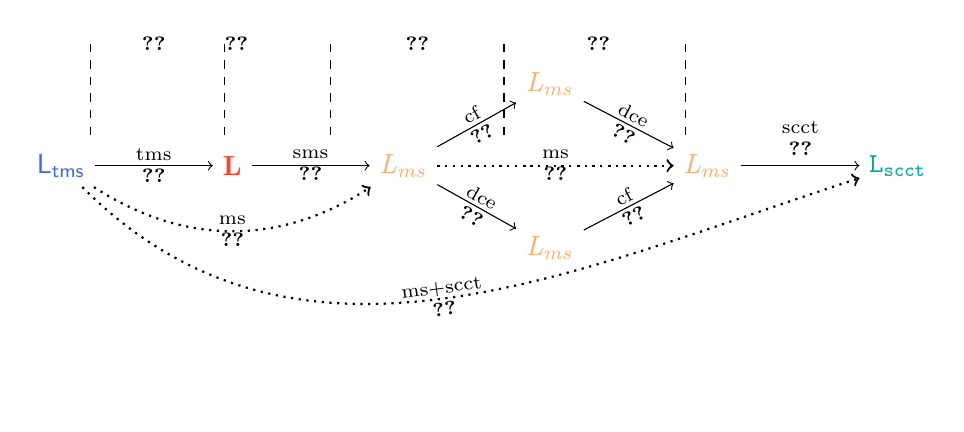
\begin{tikzpicture}
      \node (S) {$\src{L_{\tmssafe}}$};
      \node[right=1.5 of S] (T) {$\trg{L}$};
      \node[right=1.5 of T] (M) {$\irl{L_{\mssafe}}$};
      \node[below right=0.5 and 1.0 of M] (D0) {$\irl{L_{\mssafe}}$};
      \node[above right=0.5 and 1.0 of M] (C0) {$\irl{L_{\mssafe}}$};
      \node[right=3.0 of M] (E) {$\irl{L_{\mssafe}}$};
      \node[right=1.5 of E] (O) {$\obj{L_{\scctsafe}}$};

      \draw[->] (S) to[sloped] node[align=center,font=\scriptsize] (tmsedge) {\gls{tms}\\ \Cref{thm:cca:rtp:tms}} (T);
      \draw[->] (T) to[sloped] node[align=center,font=\scriptsize] {\gls{sms}\\ \Cref{thm:ccb:rtp:sms}} (M);
      \draw[->] (M) to[sloped] node[align=center,font=\scriptsize] {\gls{dce}\\ \Cref{thm:ccdce:rtp:ms}} (D0);
      \draw[->] (M) to[sloped] node[align=center,font=\scriptsize] {\gls{cf}\\ \Cref{thm:cccf:rtp:ms}} (C0);
      \draw[->] (D0) to[sloped] node[align=center,font=\scriptsize] {\gls{cf}\\ \Cref{thm:cccf:rtp:ms}} (E);
      \draw[->] (C0) to[sloped] node[align=center,font=\scriptsize] {\gls{dce}\\ \Cref{thm:ccdce:rtp:ms}} (E);
      \draw[->] (E) to[sloped,above] node[align=center,font=\scriptsize] {\gls{scct}\\ \Cref{thm:ccscct:rtp:scct}} (O);

      % Sections
      \node[above=1.0 of tmsedge] (sectms) {{\scriptsize\Cref{subsec:cs:tms}}};
      \node[right=0.5 of sectms] (secsms) {{\scriptsize\Cref{subsec:cs:ms}}};
      \node[right=1.75 of secsms] (secopts) {{\scriptsize\Cref{subsec:cs:opts}}};
      \node[right=1.75 of secopts] (secscct) {{\scriptsize\Cref{subsec:cs:scct}}};

      \draw[thick,dotted,->] (S) to[bend right=33,sloped] node[align=center,font=\scriptsize] {\gls{ms}\\ \Cref{thm:ccab:rtp:ms}} (M);
      \draw[thick,dotted,->] (M) to[bend right=0,sloped] node[align=center,font=\scriptsize] {\gls{ms}\\ \Cref{thm:cccfccdce:rtp:ms}} (E);
      \draw[thick,dotted,->] (S) to[out=-45,in=198,sloped] node[align=center,font=\scriptsize] {\gls{ms}+\gls{scct}\\ \Cref{thm:ccall:rtp:msscct}} (O);

      \draw[dashed] ($(sectms)-(0.8,0)$) -- ($(sectms)-(0.8,1.25)$);
      \draw[dashed] ($(sectms)-(-0.9,0)$) -- ($(sectms)-(-0.9,1.25)$);
      \draw[dashed] ($(secsms)-(-1.2,0)$) -- ($(secsms)-(-1.2,1.25)$);
      \draw[dashed] ($(secscct)-(1.2,0)$) -- ($(secscct)-(1.2,1.25)$);
      \draw[dashed] ($(secscct)-(-1.1,0)$) -- ($(secscct)-(-1.1,1.25)$);
    \end{tikzpicture}
  \end{center}
  \caption{Visualisation of the optimising compilation pipeline that attains a combination of \gls{ms} and \gls{cct}.}\label{fig:pipeline}
\end{figure}
This section defines several secure compilers, each of which robustly preserves a different property of interest (\Cref{fig:pipeline}).
It demonstrates the power of the framework (\Cref{sec:compprop,sec:compcomp}) by composing these compilers for a secure and optimising compilation chain that robustly preserves \gls{msscct}.
The first step in this chain is the compiler from $\src{L_{\tmssafe}}$ to $\trg{L}$ that robustly preserves just \gls{tms} (\Cref{thm:cca:rtp:tms}).
From here, an instrumentation from $\trg{L}$ to $\irl{L_{\mssafe}}$ ensures that no out-of-bounds accesses can happen and, thus, programs at this point attain \gls{sms} (\Cref{thm:ccb:rtp:sms}).
This is enough to get a compiler that robustly preserves \gls{ms} (\Cref{thm:ccab:rtp:ms}).
At this stage, the section presents two optimising translations, namely \gls{cf} and \gls{dce}, each of which robustly preserves \gls{ms} (\Cref{thm:ccdce:rtp:ms,thm:cccf:rtp:ms}).
These translations can be freely ordered in the compilation chain without compromising memory safety (\Cref{thm:cccfccdce:rtp:ms}).
The last step ensures that code stays \gls{scct} (\Cref{thm:ccscct:rtp:scct}) when lowered from $\Lms$ to $\Lscct$ which yields the final result that the whole compilation chain robustly preserves \gls{msscct} (\Cref{thm:ccall:rtp:msscct}).

\subsection{Robust Temporal Memory Safety Preservation}\label{subsec:cs:tms}

  $$
  \begin{array}{rcl}
%    \cca(\src{\lbinop{\expr[_{1}]}{\expr[_{2}]}}) & = & \lbinop[\trg]{\left[\cca(\src{\expr[_{1}]})\right]}{\left[\cca(\src{\expr[_{2}]})\right]} \\ [0.33cm]
    \cca(\src{\lfunction{g}{x:\natt\to\type[_{e}]}{\expr}}) & = & \lfunction[\trg]{\trg{g}}{\trg{x}}{\lifz[\trg]{\trg{\lhast{x}{\natt}}}{%
                                                                                                \left[\cca(\src{\expr})\right] %
                                                                                                 }{\labort[\trg]}}
  \end{array}
  $$

The compiler does not have to do anything special besides a typecheck to respect the calling-convention.
That is, because $\trg{L}$ has no static typechecks, it could happen that a bogus context $\trg{\library_{\ctx}}$ invokes a callable object accepting a $\src{\natt}$ with $\trg{\lpair{17}{29}}$.
By inserting the check, the compiler ensures that execution does not proceed in such cases.
The compiler does not insert other checks and simply recolors $\src{L_{\tmssafe}}$ to $\trg{L}$ expressions.
Hypothesizing an implementation of the \texttt{strncpy} function from \Cref{sec:introduction} in $\Ltms$, the compiler would in this case ensure that the arguments are valid.

\begin{theorem}[Compiler $\cca$ is secure with respect to \gls{tms}]\label{thm:cca:rtp:tms}
  $\rtp{\cca}{\tmssafe}$ % \Coqed
\end{theorem}

\begin{proof}[Proof Sketch]
The proof of \Cref{thm:cca:rtp:tms} uses standard techniques in secure compilation literature and is visualized in \Cref{fig:proofdiag:rtp}.
Concretely, given the execution of the compiled $\Ltms$ program linked with an arbitrary $\trg{L}$ context yields a trace $\trg{\trace}$, it uses a trace-based backtranslation of $\trg{\trace}$ to reconstruct an $\src{L_{\tmssafe}}$ context.
\Cref{thm:wt:tms} already gives strong guarantees for programs written in $\src{L_{\tmssafe}}$ and can be exploited for the backtranslated context by ensuring that it typechecks.
Well-typing means the $\src{L_{\tmssafe}}$ program runs, so the rest of the proof is about relating the $\trg{L}$-level execution with the $\src{L_{\tmssafe}}$-level execution.

For the $\trg{L}$-execution, the compiler wrapper code at state $\trg{\Omega_{1}}$ may either crash the program or continue execution $\trg{\Omega_{w_{1}}}$ right before control is transferred to the component.
In this specific case, the compiler need not to insert additional code after the component is done with its execution, but a symmetric situation can happen here.
Similarily, the backtranslation may also insert wrapper code prior and after switching to and from the component to the context.
\MKin{
  more detail or not? ;
  i.e., explain $\multimap$ and $\approx$?
}
\end{proof}

\begin{figure}[h]
  \begin{center}
    \begin{tikzpicture}[state/.style={minimum height=0.6cm}]
      % relative horizontal/vertical distance between states
      \pgfmathsetmacro{\hdist}{0.95}
      \pgfmathsetmacro{\vdist}{1.35}
      \pgfmathsetmacro{\halfvdist}{0.725}

      % row of src states
      \node[state] (srcempty) {$\src{\emptyset}$};
      \foreach \s [remember=\s as \cur (initially empty)] in {1,w_1,p,w_2,2} {
        \node[state,right=\hdist of src\cur] (src\s) {$\src{\Omega_{\s}}$};
      }
      % row of trg states
      \node[state,below=\vdist of srcempty] (trgempty) {$\trg{\emptyset}$};
      \foreach \s in {1,w_1,p,w_2,2} {
        \node[state,below=\vdist of src\s] (trg\s) {$\trg{\Omega_{\s}}$};
      }
      %% illustrations
        % backtrans wrapper 1
        \draw[thick,loosely dotted,Peach!50,rounded corners] (src1.north east) -- (srcw\string_1.north east)
          -- (trgw\string_1.south east) -- (trg1.south west) -- (src1.north west) -- cycle;
        % backtrans wrapper 2
        \draw[thick,loosely dotted,Peach!50,rounded corners] (srcp.north east) -- (srcw\string_2.north east)
          -- (trgw\string_2.south east) -- (trgp.south west) -- (srcp.north west) -- cycle;
        % compiler correctness
        \draw[thick,loosely dashed,Emerald!50,rounded corners] ($(srcw\string_1.north east)+(0,0.05)$) -- ($(srcp.north east)+(0,0.05)$)
          -- ($(trgw\string_2.north east)+(0.05,0)$) -- ($(trgw\string_2.south east)+(0.05,-0.05)$)
          -- ($(trg1.south west)+(-0.05,-0.05)$) -- ($(trg1.north west)+(-0.05,0)$) -- ($(srcw\string_1.north west)+(0,0.05)$) -- cycle;
      % state relations
      \path (srcempty) edge[draw=gray!25] node[pos=0.5,sloped,rotate=180,fill=white] {\scriptsize$\multimap_\emptyset$} (trgempty)
        (src1) edge[draw=gray!25] node[pos=0.5,sloped,rotate=180,fill=white] {\scriptsize$\multimap_{\delta_1}$} (trg1)
        (srcp) edge[draw=gray!25] node[pos=0.5,sloped,fill=white] {\scriptsize$\approx_{\delta_p}$} (trgp)
        (src2) edge[draw=gray!25] node[pos=0.5,sloped,rotate=180,fill=white] {\scriptsize$\multimap_{\delta_2}$} (trg2)
        (srcw\string_1) edge[draw=gray!25] node[pos=0.5,sloped,fill=white] {\scriptsize$\approx_{\delta_{w_1}}$} (trgw\string_1)
        (srcw\string_2) edge[draw=gray!25] node[pos=0.5,sloped,rotate=180,fill=white] {\scriptsize$\multimap_{\delta_{w_2}}$} (trgw\string_2)
        % diagonals
        (srcw\string_1) edge[draw=gray!25] node[pos=0.16,sloped,rotate=180,fill=white] {\scriptsize$\approx_{\delta_{w_1}}$} (trg1)
        (src1) edge[draw=gray!25] node[pos=0.16,sloped,rotate=180,fill=white] {\scriptsize$\multimap_{\delta_1}$} (trgw\string_1)
        (srcp) edge[draw=gray!25] node[pos=0.2,sloped,fill=white] {\scriptsize$\approx_{\delta_p}$} (trgw\string_2)
        (trgp) edge[draw=gray!25] node[pos=0.2,sloped,fill=white] {\scriptsize$\multimap_{\delta_{w_2}}$} (srcw\string_2)
        ;
      %\drawpolygon src1,srcw\string_1,trgw\string_1,trg1;
      %\drawpolygon srcp,srcw\string_2,trgw\string_2,trgp;
      %\node[font=\tiny,align=center,above=0.2 of srcw1srcp] (wrapper) {Backtranslation\\Wrapper};
      %\path[->,draw] (wrapper) -- (srcw\string_1);
      %\path[->,draw] (wrapper) -- (srcp);
      % steps
      \path[color=\stlccol] (srcempty) edge[draw=none] node {\ $\xrightarrow{\trace[_1]}{}{\kern-3.5pt}_{\text{ctx}}^*$} (src1)
        (src1) edge[draw=none] node {\ $\xrightarrow{\trace[_c]}{}{\kern-3.5pt}_{\text{ctx}}$} (srcw\string_1)
        (srcw\string_1) edge[draw=none] node {\ $\xrightarrow{\trace[_p]}{}{\kern-3.5pt}_{\text{ctx}}^*$} (srcp)
        (srcp) edge[draw=none] node[fill=white,inner sep=0,outer sep=0] {\ $\xrightarrow{\trace[_r]}{}{\kern-3.5pt}_{\text{ctx}}$} (srcw\string_2)
        (srcw\string_2) edge[draw=none] node {\ $\xrightarrow{\trace[_2]}{}{\kern-3.5pt}_{\text{ctx}}^*$} (src2)
        ;
      \path[color=\ulccol] (trgempty) edge[draw=none] node[fill=white,inner sep=0,outer sep=0] {\ $\xrightarrow{\phantom{\trace[_1]}}{}{\kern-3.5pt}_{\text{ctx}}^*$} (trg1)
        (trg1) edge[draw=none] node {\ $\xrightarrow{\phantom{\trace[_p]}}{}{\kern-3.5pt}_{\text{ctx}}^*$} (trgw\string_1)
        (trgw\string_1) edge[draw=none] node[fill=white,inner sep=0,outer sep=0] {\ $\xrightarrow{\phantom{\trace[_p]}}{}{\kern-3.5pt}_{\text{ctx}}^*$} (trgp)
        (trgp) edge[draw=none] node {\ $\xrightarrow{\phantom{\trace[_p]}}{}{\kern-3.5pt}_{\text{ctx}}^*$} (trgw\string_2)
        (trgw\string_2) edge[draw=none] node {\ $\xrightarrow{\phantom{\trace[_2]}}{}{\kern-3.5pt}_{\text{ctx}}^*$} (trg2)
        ;
      % legend
      \node[align=left,below right=0.3 and 0.3 of trgempty,font=\tiny] (legend) {%
        ${\src{\trace[_c]}}\cong{\backt{\Ltms}{\Ltrg}(\trg{Call\ ?\ foo\ \valueexpr})}$\\%
        ${\src{\trace[_r]}}\cong{\backt{\Ltms}{\Ltrg}(\trg{Ret\ !\ foo\ \valueexpr})}$
        };
      \draw[thick,loosely dotted,Peach!50,rounded corners] ($(legend.north east)+(0.5,-0.4)$) -- ($(legend.north east)+(1,-0.4)$);
      \node at ($(legend.north east)+(1.5,-0.4)$) (legendwrapper) {};
      \node[right of=legendwrapper] {\tiny Backtranslation Wrapper};
      \draw[thick,loosely dashed,Emerald!50,rounded corners] ($(legend.south east)+(0.5,0.4)$) -- ($(legend.south east)+(1,0.4)$);
      \node at ($(legend.south east)+(1.5,0.4)$) (legendcorrectness) {};
      \node[right of=legendcorrectness] {\tiny Compiler Correctness};
    \end{tikzpicture}
    \caption{Proof diagram for \Cref{thm:cca:rtp:tms} depicting the general structure of robust preservation proofs.}\label{fig:proofdiag:rtp}
  \end{center}
\end{figure}

\subsection{Robust (Spatial) Memory Safety Preservation}\label{subsec:cs:ms}

\begin{center}
  $$
  \begin{array}{rcl}
    \ccb(\trg{\lnew{x}{\expr[_{1}]}{\expr[_{2}]}}) & = & \llet[\irl]{\irl{x_{SIZE}}}{\ccb(\trg{\expr[_{1}]})}{\lnew[\irl]{\irl{x}}{\irl{x_{SIZE}}}{\ccb(\trg{\expr[_{2}]})}} \\
    \ccb(\trg{\lget{x}{\expr}}) & = & \llet[\irl]{\irl{x_{n}}}{\ccb(\trg{\expr})}{\irl{\lifz{0\le x_{n}<x_{SIZE}}{\lget{x}{x_{n}}}{\labort}}} \\
    \ccb(\trg{\lset{x}{\expr[_{1}]}{\expr[_{2}]}}) & = & \llet[\irl]{\irl{x_{n}}}{\ccb(\trg{\expr[_{1}]})}{\lifz[\irl]{\irl{0\le x_{n}<x_{SIZE}}}{\lset[\irl]{\irl{x}}{\irl{x_{n}}}{\ccb(\trg{\expr[_{2}]})}}{\irl{\labort}}} \\
  \end{array}
  $$
\end{center}

Up to getting and setting memory, the compiler is the identity function, i.e., all omitted cases are a recoloring of $\trg{L}$ to $\Lms$.
For memory accesses, however, a bounds-check is inserted that enforces \gls{sms}.
To this end, the compiler introduces another, fresh identifier $\irl{x_{SIZE}}$ for each allocation that binds $\irl{x}$ to keep track of the allocation size.
Again, linking this back to the \texttt{strncpy} example corresponds to the insertion of bounds check right in front of the accesses to \texttt{y[i]} and \texttt{x[i]}.

\begin{theorem}[Compiler $\ccb$ is secure with respect to \gls{sms}]\label{thm:ccb:rtp:sms}
  $\rtp{\ccb}{\smssafe}$ % \Coqed
\end{theorem}

It is now possible to make use of \Cref{thm:rtp} to extract a compiler from $\Ltms$ to $\Lms$ that is \gls{ms} by applying \Cref{thm:cca:rtp:tms,thm:ccb:rtp:sms}:

\begin{theorem}[Compiler $\cca\circ\ccb$ is secure with respect to \gls{ms}]\label{thm:ccab:rtp:ms}
  $\rtp{\cca\circ\ccb}{\mssafe}$ % \Coqed
\end{theorem}

\subsection{Optimising Compilers}\label{subsec:cs:opts}

\begin{center}
  $$
  \begin{array}{rcl}
    \ccdce(\irl{\lifz{true}{\expr[_{1}]}{\expr[_{2}]}}) & = & \ccdce(\irl{\expr[_{1}]}) \\
    \ccdce(\irl{\lifz{false}{\expr[_{1}]}{\expr[_{2}]}}) & = & \ccdce(\irl{\expr[_{2}]}) \\
  \end{array}
  $$
\end{center}

\begin{center}
  $$
  \begin{array}{rcll}
    \cccf(\irl{\llet{x}{n}{\expr}}) & = & \cccf(\irl{\expr\subst{n}{x}}) &\\
    \cccf(\irl{\lbinop{n_{1}}{n_{2}}}) & = & \irl{n_{3}} & \text{where }\irl{n_{3}}\text{ is }\lbinop{\irl{n_{1}}}{\irl{n_{2}}}\\
  \end{array}
  $$
\end{center}

The two optimising compiler passes from $\Lms$ to $\Lms$ perform \gls{dce} and \gls{cf}, respectively.
Both are secure with respect to \gls{ms}, the proof of which is relatively easy, since the backtranslation can use the original context without modification and both transformations do not change anything with regards to allocation, use, or deallocation.
That is, the order of appearance of the events on the execution trace stays the same.

\begin{theorem}[Compiler $\ccdce$ is secure with respect to \gls{ms}]\label{thm:ccdce:rtp:ms}
  $\rtp{\ccdce}{\mssafe}$ % \Coqed
\end{theorem}
\begin{theorem}[Compiler $\cccf$ is secure with respect to \gls{ms}]\label{thm:cccf:rtp:ms}
  $\rtp{\cccf}{\mssafe}$ % \Coqed
\end{theorem}

With both \Cref{thm:ccdce:rtp:ms,thm:cccf:rtp:ms} it follows from \Cref{corr:swappable} that the two passes can be interchanged arbitrarily:

\begin{theorem}[Compilers $\cccf\circ\ccdce$ and $\cccf\circ\ccdce$ are secure with respect to \gls{ms}]\label{thm:cccfccdce:rtp:ms}
  $\rtp{\cccf\circ\ccdce}{\mssafe}$ and $\rtp{\ccdce\circ\cccf}{\mssafe}$ % \Coqed
\end{theorem}

\subsection{Robust Strict Cryptographic Constant Time Preservation}\label{subsec:cs:scct}

\begin{center}
  $$
  \begin{array}{rcl}
    \ccscct(\irl{\lfunction{g}{x}{\expr}}) & = & \lfunction[\obj]{\obj{g}}{\obj{x}}{\obj{\lwrdoit{1};}\ccscct(\irl{\expr})}
  \end{array}
  $$
\end{center}

Given the fact that $\Lscct$ provides a \gls{cct}-mode, the compiler has to ensure that execution in the component always happen in this mode.
The context could overwrite the flag and exit the mode, but upon invoking a callable object that is part of the component, the flag would be set again.
Because of this, the compiler is secure with respect ot \gls{scct}, similarily proven as in \Cref{subsec:cs:tms}.

\begin{theorem}[Compiler $\ccscct$ is secure with respect to \gls{scct}]\label{thm:ccscct:rtp:scct}
  $\rtp{\ccscct}{\scctsafe}$ % \Coqed
\end{theorem}

\subsection{Robust Preservation of Intersection of Memory Safety and Strict Cryptographic Constant Time}

Let $\ccmsscct$ be the compiler that is the composition of $\cca$, $\ccb$, $\cccf$, $\ccdce$, and $\ccscct$, then the following theorem can be shown.

\begin{theorem}[Compiler $\ccmsscct$ is secure with respect to \gls{scct}]\label{thm:ccall:rtp:msscct}
  $\rtp{\cc{\Ltms}{\Lscct}}{\mssafe\cap\scctsafe}$ % \Coqed
\end{theorem}

%\begin{lstlisting}[language=c,caption=``Wrong bounds check of two 64-bit integers.'']
%if at <= bounds {
%  x[at] = 42;
%}
%\end{lstlisting}
%Note the subtle bug of using \verb|<=| instead of \verb|<|, leading to an out-of-bounds access whenever \verb|at = bounds|.
%Furthermore, when \verb|at| and \verb|bounds| are 64-bit integers on a 32-bit architecture, the comparison may not be performed in constant-time: The compiler may bail out as soon as the lower 32 bits are unequal, not bothering to compare the higher 32 bits.


\section{Related Work\pages{2}}\label{sec:relwork}

This section compares existing work with the one presented in this paper.
To this end, work on robust preservation (\Cref{subsec:relw:seccomprtp}) and on other secure compiler criteria (\Cref{subsec:relw:seccompcrit}) is looked at.
The case study of this paper (\Cref{sec:casestud:defs,sec:casestud:rtp}) implements measures for ensuring \gls{ms} as well as \gls{cct} and these are compared with previous work as well (\Cref{subsec:relw:msmechs,subsec:relw:cctmechs}).

\subsection{Secure Compilation as Robust Preservation}\label{subsec:relw:seccomprtp}

The robust preservation of properties as a compiler-level criterion has been analyzed extensively~\cite{abate2019jour,patrignani2021rsc,abate2021extacc,patrignani2022universal,patrignani2019survey,kruse2022csc}.
This work has made use of that previous work.
While there exists a composition theorem~\cite{abate2019jour} already, that theorem is not concerned with composing robustly safe compilers, but rather program components and contexts.
The work relating robust preservation with universal composability~\cite{patrignani2022universal} is closest to what this paper presents.
The authors demonstrate a similar compositionality theorem to what is presented here (\Cref{sec:compcomp}) as well as in an earlier version of this work~\cite{kruse2022csc}.
However, they do not demonstrate the scalability of the approach by means of a case study.

\subsection{Other Secure Compilation Criteria}\label{subsec:relw:seccompcrit}

While this paper focuses on the robust preservation framework~\cite{abate2019jour}, other secure compilation criteria exist.
The survey on formal approaches to secure compilation~\cite{patrignani2019survey} discusses a broad spectrum already, while this section presents a very high-level overview.
The full abstraction approach~\cite{abadi1999fullabstraction} states that a compiler should preserve and reflect observational equivalence between source and target programs.
It was shown~\cite{abate2021faandrc} that fully abstract compilers robustly preserve program properties that are either trivial or meaningless.
As a mitigation for this, the authors presented a categorical approach based on maps of distributive laws~\cite{watanabe2002modl}, which they call many maps of distributive laws.
Maps of distributive laws have been investigated before as a possible secure compilation criterion~\cite{tsampas2020catsc}.
Other approaches are extensions of the compiler correctness criterion as discussed in other work~\cite{patterson2019next700} or the introduction of opaque observations~\cite{vu2021reconciling} to reconcile compiler optimisations with security.
Note that this work also presents secure compilers that are optimising, but contrary to the other~\cite{vu2021reconciling}, provides a formal account of these in the robust preservation framework.
Lastly, the authors of this paper have presented ongoing work~\cite{patrignani2023blame} on a weaker robust preservation criteria based on the concept blame.

\subsection{Memory Safety Mechanisms}\label{subsec:relw:msmechs}

Different mechanisms for memory safety exist that also consider the secure compilation domain, i.e., have an active attacker model.
For example, the ,,pointers as capabilities'' principle represents pointers as machine-level capabilities~\cite{korashy2021capableptrs}, which behave in a similar fashion to capabilities by means of linear typing~\cite{morrisett2005L3}.
The approach of this paper also uses linear typing, but differs from $L^{3}$~\cite{morrisett2005L3} in the way that functions are not first-class.
Moreover, this paper considers an active attacker, while the work on $L^{3}$ only discusses whole programs and, thus, has no active attacker model.
The instrumentation to ensure memory safety that this paper presents is inspired by seminal work in the literature~\cite{nagarakatte2009soft}.
That work inserts bounds-checks in front of pointer-dereferences and, for this to work, inserts meta-data information on pointer creation.
It also works in a more advanced setting with structured fields accesses and also introduces a table-lookup for pointers that are stored in memory.
This paper only considers pointers to arrays of simple objects, i.e., there are no pointers to pointers or structures.
Of course, there are a lot of other approaches to memory-safety in literature, specifically as compiler instrumentations~\cite{akritidis2009baggy,younan2010paricheck,jung2021pico,shankaranarayana2023tailcheck,dhumbumroong2020boundwarden,nam2019framer,zhou2023fatptrs}, hardware-extensions~\cite{kwon2013lowfat,saileshwar2022heapcheck,chen2023flexpointer,kim2023whistle}, or programming language extensions~\cite{elliott2018checkedc,li2022formalcheckedc,jim2002cyclone,elliott2015guilt,west2005cuckoo,weis2019fyr,benoit2019uniqueness}, to name a few.
What differentiates this work from them is that this work uses known, compiler-based approaches to ensure memory-safety as a means to investigate secure compiler compositions.
This paper does not provide efficient memory-safety, but serves as a theoretical foundation for the secure compilation domain.

To extend the languages in this paper with a less restricted form of pointer arithmetic, the region coloring memory safety monitor presented in earlier work~\cite{michael2023mswasm} can be used.
The work presenting this monitor provides an approach for the robust preservation of memory safety compiling from C to WASM.
However, they do not discuss composition of secure compilers but rather investigate an instance of a secure compiler.

\subsection{Cryptographic Constant Time Mechanisms}\label{subsec:relw:cctmechs}

The approach to cryptographic constant time in this paper is high-level, where a programming language exposes a way to switch the semantics to a data (operand) independent timing mode.
Since identifiers in $\Lscct$ are annotated with a secrecy tag, this approach is similar to others with information flow control.
For example, Vale~\cite{bond2017vale} uses Dafny to ensure constant-time assembly code, while Jasmin~\cite{almeida2017jasmin} makes use of the Coq proof assistant to reject non-constant-time programs.
CT-Wasm~\cite{watt2019ctwasm} enforces constant-timeness by means of a type system.
Different to the approach of this paper, these approaches necessitate that the programmer writes \gls{cct} code.
An approach to allow programmers to write more high-level code is CryptOpt~\cite{kuepper2023cryptopt}, which generates efficient target-code by means of a randomized search.
This paper abstracts over concrete mitigation strategies and simply assumes that there is a flag to switch to a cryptographic-constant time execution mode.
This can be realized by employing the FaCT~\cite{cauligi2019fact} compiler, which translates common non-constant time code patterns to be constant-time, and the data (object) independent timing execution mode of modern processors.

\section{Conclusion\pages{$\sfrac{1}{2}$}}\label{sec:concl}

This paper does a first step towards practical secure compilation chains by introducing a theoretical framework demonstrating that secure compilers compose.
The paper exercises this framework on a case-study that consists of an optimising compilation chain that is secure with respect to \gls{msscct}.
In future work, it would be interesting to investigate whether it is possible to provide {\em secure compiler combinators}, similarily to how parser combinators work.
%To this end, it may be necessary to extend existing frameworks for multi-language semantics.
It is also interesting to extend our case-study and verify all results of it in Coq.
This way, it is possible to obtain an executable, secure compiler.
However, the formalization effort for backtranslation proofs is known to be enormous, so another research avenue may be to find better ways to (semi-)automate standard secure compilation proofs.

%% The acknowledgments section is defined using the "acks" environment
%% (and NOT an unnumbered section). This ensures the proper
%% identification of the section in the article metadata, and the
%% consistent spelling of the heading.
\begin{acks}
  We would like to thank the anonymous reviewers for their feedback.
\end{acks}

%%
%% The next two lines define the bibliography style to be used, and
%% the bibliography file.
\bibliographystyle{ACM-Reference-Format}
\bibliography{main}

%%
%% If your work has an appendix, this is the place to put it.
\appendix

\end{document}
\endinput
%%
%% End of file `sample-sigconf.tex'.
